%% 
%% Copyright 2007-2024 Elsevier Ltd
%% 
%% This file is part of the 'Elsarticle Bundle'.
%% ---------------------------------------------
%% 
%% It may be distributed under the conditions of the LaTeX Project Public
%% License, either version 1.3 of this license or (at your option) any
%% later version.  The latest version of this license is in
%%    http://www.latex-project.org/lppl.txt
%% and version 1.3 or later is part of all distributions of LaTeX
%% version 1999/12/01 or later.
%% 
%% The list of all files belonging to the 'Elsarticle Bundle' is
%% given in the file `manifest.txt'.
%% 
%% Template article for Elsevier's document class `elsarticle'
%% with numbered style bibliographic references
%% SP 2008/03/01
%% $Id: elsarticle-template-num.tex 249 2024-04-06 10:51:24Z rishi $
%%
\documentclass[preprint,12pt,authoryear]{elsarticle}

%% Use the option review to obtain double line spacing
%% \documentclass[authoryear,preprint,review,12pt]{elsarticle}

%% Use the options 1p,twocolumn; 3p; 3p,twocolumn; 5p; or 5p,twocolumn
%% for a journal layout:
%% \documentclass[final,1p,times]{elsarticle}
%% \documentclass[final,1p,times,twocolumn]{elsarticle}
%% \documentclass[final,3p,times]{elsarticle}
%% \documentclass[final,3p,times,twocolumn]{elsarticle}
%% \documentclass[final,5p,times]{elsarticle}
%% \documentclass[final,5p,times,twocolumn]{elsarticle}

%% For including figures, graphicx.sty has been loaded in
%% elsarticle.cls. If you prefer to use the old commands
%% please give \usepackage{epsfig}

%% The amssymb package provides various useful mathematical symbols
\usepackage{amssymb}
%% The amsmath package provides various useful equation environments.
\usepackage{amsmath}
%% The amsthm package provides extended theorem environments
%% \usepackage{amsthm}
\usepackage{amsmath,amsfonts}
\usepackage{amssymb}
\usepackage{bm}
\usepackage{algorithm}
\usepackage{array}
\usepackage{textcomp}
\usepackage{stfloats}
\usepackage{url}
\usepackage{verbatim}
\usepackage{graphicx}
\usepackage{xcolor}
\usepackage{cite}  
\hyphenation{op-tical net-works semi-conduc-tor IEEE-Xplore}
\usepackage{algpseudocode}
\usepackage{tikz}
\usepackage{float}
\usepackage{booktabs}
\usepackage{subcaption}
\usepackage[margin=1in]{geometry}
\usepackage{tabularx}
\usepackage{amsthm}
\newtheorem{remark}{Remark}
\newtheorem{corollary}{Corollary}
\newtheorem{theorem}{Theorem}         
\newtheorem{proposition}{Proposition}  
\newtheorem{lemma}{Lemma}          
\theoremstyle{definition}
\newtheorem{definition}{Definition}   
  
\usepackage{multirow}

\newcommand{\Halmos}{\hfill$\square$}


\RequirePackage{endnotes}
%% The lineno packages adds line numbers. Start line numbering with
%% \begin{linenumbers}, end it with \end{linenumbers}. Or switch it on
%% for the whole article with \linenumbers.
%% \usepackage{lineno}

\journal{Transportation Research Part E: Logistics and Transportation Review}

\begin{document}

\begin{frontmatter}

%% Title, authors and addresses

%% use the tnoteref command within \title for footnotes;
%% use the tnotetext command for theassociated footnote;
%% use the fnref command within \author or \affiliation for footnotes;
%% use the fntext command for theassociated footnote;
%% use the corref command within \author for corresponding author footnotes;
%% use the cortext command for theassociated footnote;
%% use the ead command for the email address,
%% and the form \ead[url] for the home page:
%% \title{Title\tnoteref{label1}}
%% \tnotetext[label1]{}
%% \author{Name\corref{cor1}\fnref{label2}}
%% \ead{email address}
%% \ead[url]{home page}
%% \fntext[label2]{}
%% \cortext[cor1]{}
%% \affiliation{organization={},
%%             addressline={},
%%             city={},
%%             postcode={},
%%             state={},
%%             country={}}
%% \fntext[label3]{}

\title{
Distributionally Robust Prize-Collecting Vehicle Routing based on Observation Data
}

%% use optional labels to link authors explicitly to addresses:
%% \author[label1,label2]{}
%% \affiliation[label1]{organization={},
%%             addressline={},
%%             city={},
%%             postcode={},
%%             state={},
%%             country={}}
%%
%% \affiliation[label2]{organization={},
%%             addressline={},
%%             city={},
%%             postcode={},
%%             state={},
%%             country={}}



%% Abstract
\begin{abstract}



Vehicle routing problems (VRP) and their variants, such as team orienteering problems and prize-collecting VRPs, typically assume that service locations and prizes are known before optimization. However, in observation-driven applications such as environmental inspection, emergency response, and humanitarian relief, candidate locations and their uncertain prizes often need to be inferred from massive and noisy observation data. Here, prize refers to the expected benefit of visiting a node, such as inspection value, risk-reduction value, or service benefit, depending on the application context. 
To this end, this paper develops an observation-driven data pipeline and integrated solution framework with a two-stage distributionally robust prize-collecting vehicle routing problem (DR-PCVRP). 
The first stage devises an adaptive dynamic clustering algorithm to aggregate spatially concentrated observations into candidate nodes with empirical prize samples, achieving expected amortized $O(\log^4 m)$ per-update complexity for fixed-dimensional spatial data, where $m$ denotes the current clustering data size. The second stage characterizes prize uncertainty through a Wasserstein ambiguity set and develops a hybrid solution framework that combines deep-reinforcement-learning-based warm starts with neighborhood-search refinement. Experiments on standard test datasets demonstrate the effectiveness of the proposed clustering algorithm and hybrid routing algorithm in terms of solution quality and computational efficiency, particularly for large-scale instances. The results show that the framework can efficiently construct candidate nodes from large-scale observations and generate robust routes evaluated under the exact Wasserstein DRO objective. Finally, a real-world case study of urban environmental management involving more than 100 million GPS records in Chengdu confirms the framework's scalability and practical applicability, with the Exact DRO solution achieving the lowest mean out-of-sample loss compared with stochastic programming and robust optimization.

\end{abstract}


%The second stage formulates the DR-PCVRP using a Wasserstein ambiguity set to characterize prize uncertainty and develops a hybrid solution framework based on deep reinforcement learning, which substantially reduces blind exploration through learning transferable structural patterns and rapidly generating high-quality warm-start solutions, effectively achieving rapid convergence. 

%Experimental results on benchmark instances derived from CVRPLIB show that the proposed hybrid algorithm achieves substantially lower optimality gaps than learning-based baselines within comparable runtimes, and attains near-optimal solutions with gaps below 6.03\% on large-scale instances within 10 seconds, while classical Hybrid Genetic Search (HGS) with the same time fails to produce feasible solutions.

%%Graphical abstract
%\begin{graphicalabstract}
%\includegraphics{grabs}
%\begin{figure*}[htbp]
%    \centering
%    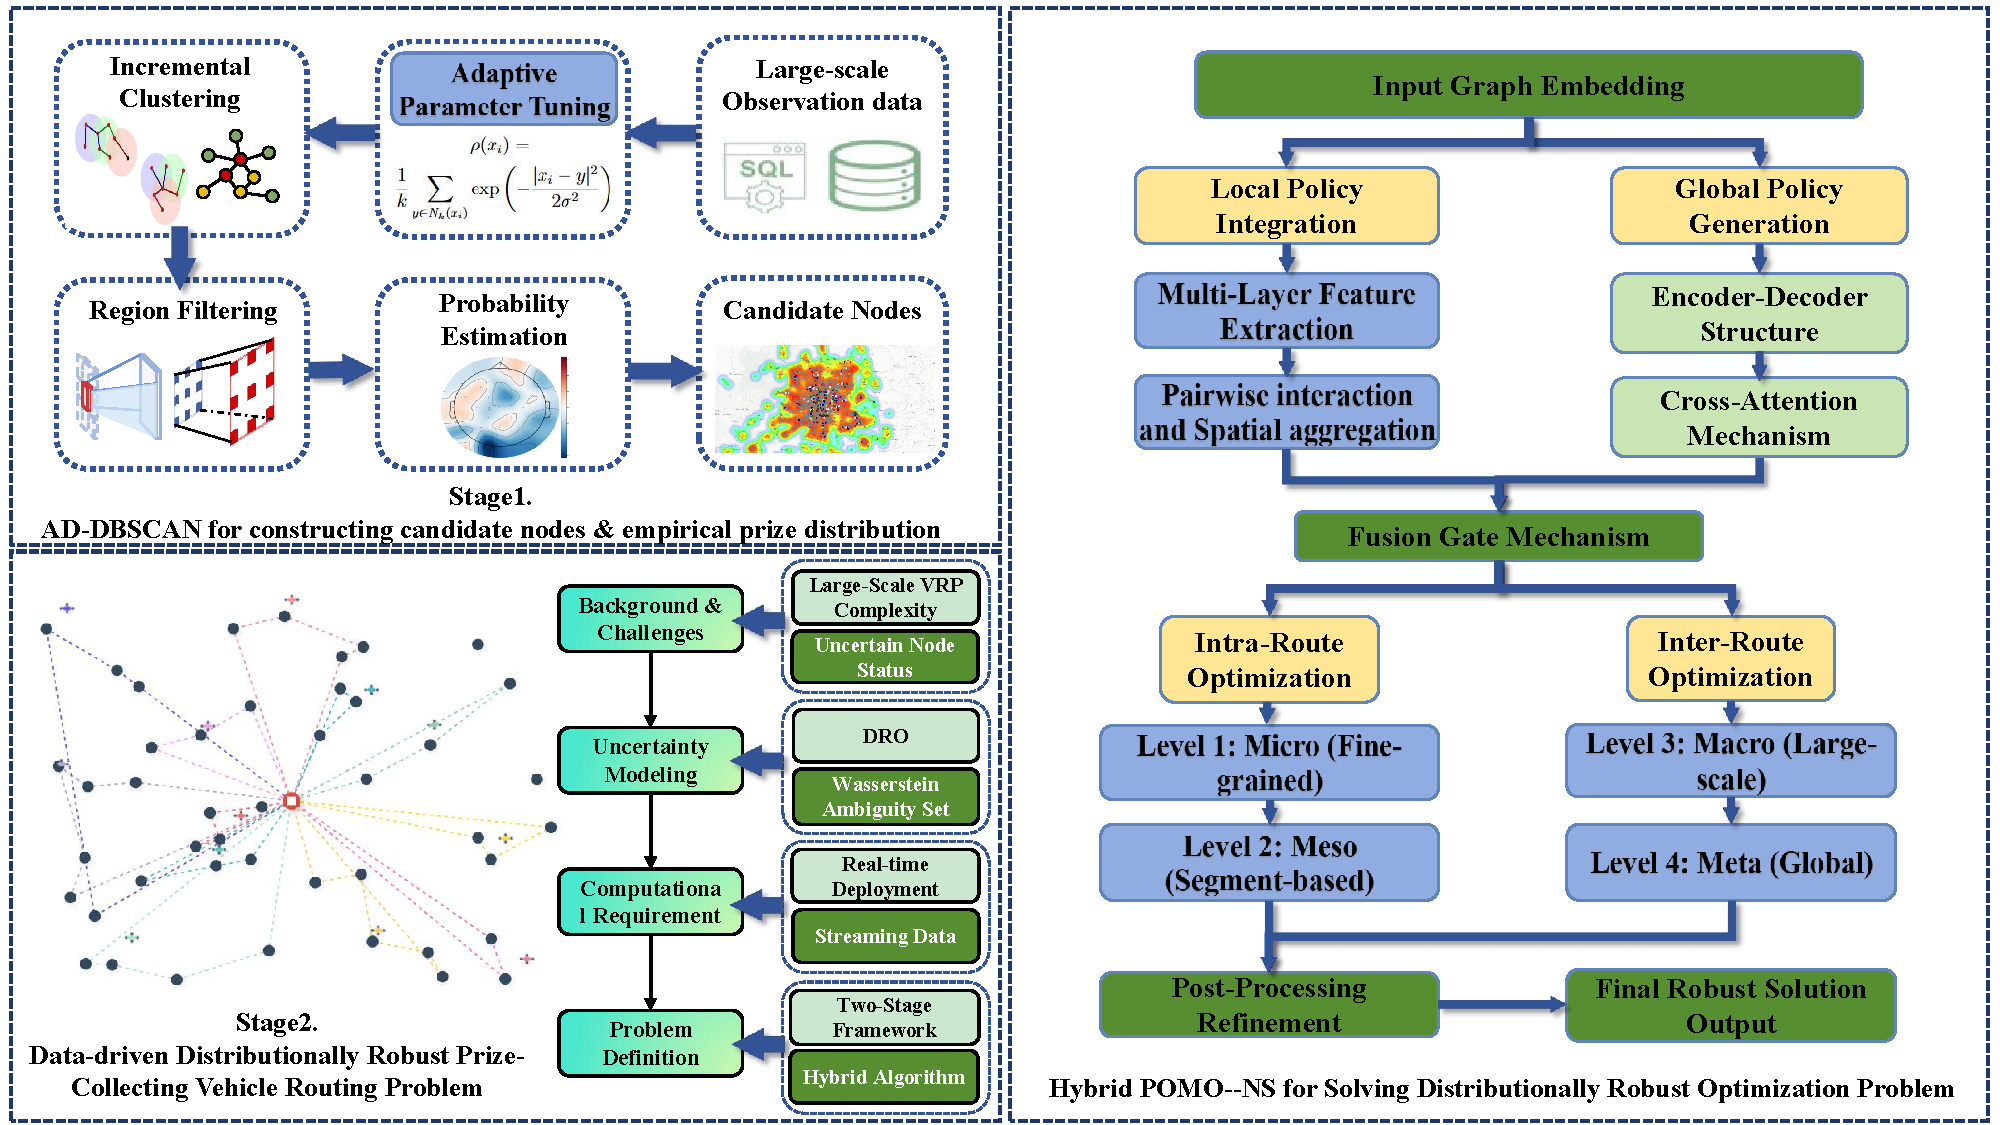
\includegraphics[width=\textwidth]{Graphical Abstract.pdf}    
%\end{figure*}
%\end{graphicalabstract}

%%Research highlights
%% Keywords
\begin{keyword}
%% keywords here, in the form: keyword \sep keyword
Distributionally Robust Optimization \sep Reinforcement Learning \sep Adaptive Dynamic Clustering \sep Hybrid Optimization Algorithm \sep
Vehicle Routing under Uncertainty.
%% PACS codes here, in the form: \PACS code \sep code

%% MSC codes here, in the form: \MSC code \sep code
%% or \MSC[2008] code \sep code (2000 is the default)

\end{keyword}

\end{frontmatter}

\section{Introduction}\label{sec:Intro}


The Vehicle Routing Problem (VRP) and its variants present fundamental combinatorial optimization challenges with wide-ranging applications in logistics, transportation, and service operations \citep{eksioglu2009vehicle, konstantakopoulos2022vehicle,zhang2021robust}. Classical VRPs  typically assume the service locations and prizes to be known in advance. In certain routing applications, however, such information may not be given a priori, but can be constructed from massive, unlabeled observation data, such as GPS trajectories, sensor readings, or behavioral patterns. Scenarios fitting this category include infrastructure inspection \citep{pan2024unmanned}, environmental monitoring \citep{cirovic2014green}, predictive maintenance \citep{gerum2019data} and emergency response \citep{zografos2008decision}, where a large number of potential service locations and their associated prizes are suggested by empirical data, while limited routing capacity precludes formulation of a classical routing problem over all potential locations. 

In such settings, a principled mechanism is required to construct candidate nodes from observations and to prioritize them based on spatial concentration and inferred service urgency  \citep{shehadeh2023distributionally}. Intuitively, observations clustered in high-density regions signal elevated importance, as persistent spatial patterns often reflect systematic phenomena requiring attention \citep{yin2024wasserstein}. Throughout this paper, we consider {\it prize} to be the benefit obtained by visiting a candidate node. In the case of urban environmental management (Figure \ref{fig:CR}), the prize is interpreted as the benefit of environmental inspection: stronger aggregation of construction-waste trucks indicates a higher likelihood of on-going earthworks, with associated risks of particulate matter emissions, illegal dumping, and disturbance to the general public, which are all positively correlated with the concentrations of GPS points. Therefore, from the perspective of environmental and urban management, visiting these locations by inspectors or law enforcement units has a greater chance of mitigating these environmental risks.  By exploiting this spatial structure through density-based clustering, massive observation data are aggregated into a set of representative high-priority candidate nodes, each associated with an inferred prize that exhibits uncertainty \citep{gupta2012approximation, yu2022improving}. This yields a PCVRP with data-driven node identification and prize uncertainty characterization. Figure \ref{fig:CR} provides a real-world example of such a routing problem, in the context of urban environmental management. Solving such problems demands the ability to process large-scale data in a timely fashion, and routing techniques that remain robust under distributional ambiguity. Nevertheless, current approaches generally fail to satisfy these two requirements concurrently \citep{costa2019exact}.

\begin{figure}[htbp]
    \centering
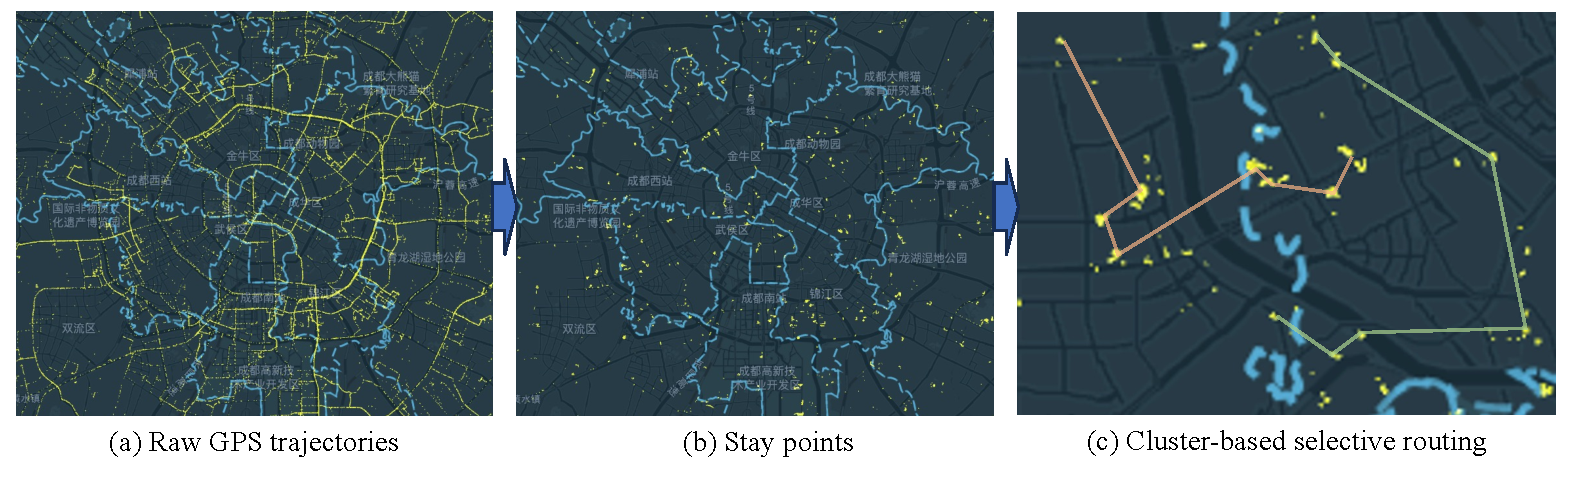
\includegraphics[width=\linewidth]{clusterrouting.pdf}
    \caption{{A representative application of observation-driven selective routing. According to Chengdu's Heavy Pollution Emergency Response Plan, during heavy pollution episodes, all on-going earthwork projects (e.g. construction and waste disposal) should be halted or conducted discreetly with pollution mitigation measures. In this case, environmental law enforcement units rely on GPS data of construction waste trucks as indicators of on-going earthwork activities to conduct selective routing and on-site inspection. (a) Raw GPS data of construction-waste trucks for a period of one hour in Chengdu, China. (b) Stay points, characterized as GPS points associated with idle or slow movement \citep{yu2025using}, signal earthwork activities associated with environmental risks. (c) Two candidate routes, to be generated in real time, that selectively visit stay point clusters, which are nodes with prize uncertainty derived using the proposed methods.}}
    \label{fig:CR}
\end{figure}




Specifically, there are two major challenges when establishing an effective solution framework. 
First, identifying candidate nodes from massive observation data incurs high computational costs, urging efficient clustering algorithms to support timely updates. 
However, existing large-scale clustering algorithms mostly employ hash functions for dimensionality reduction, struggling to maintain effective clustering structures in low-dimensional spaces \citep{shin2025dynamic}. 
Second, robust, stochastic, risk-averse and dynamic prize-collecting or orienteering variants already address several forms of prize uncertainty \citep{marinakis2013particle,secomandi2009reoptimization,zhang2012scatter,wang2025sinkhorn}. 
The challenge considered in the present study is even narrower: the candidate nodes and joint prize samples must first be constructed from a massive observation stream and then propagated consistently into a tractable robust routing objective. 
Nevertheless, exact algorithms become difficult to scale to this integrated setting \citep{costa2019exact}, traditional metaheuristics require repeated costly objective evaluations \citep{liu2025conditional}, and deep reinforcement learning offers fast construction but does not by itself provide exact distributionally robust evaluation \citep{bai2023analytics,pan2023deep,mesa2025machine}.



These observations indicate three limitations. 
First, most prize-collecting and orienteering-type routing models treat candidate nodes and prizes as exogenous inputs, while in many real-world cases such information has to be derived from empirical data, which has a subsequent impact on routing performance. 
Second, studies on robust or distributionally robust VRP variants mainly focus on uncertain demand, travel time, or service time, whereas uncertainty in the node prizes has received limited attention. 
Third, scalable clustering, robust optimization and learning-based routing algorithms are often developed as separate routines. 
As a result, uncertainty information extracted from raw observations is not systematically propagated into robust routing decisions.


Accordingly, the main contributions of this study are summarized below.


\begin{itemize} 
\item \textbf{Observation-to-routing integration:} We develop a two-stage framework that transforms spatial observations into candidate nodes and joint prize samples, which are used to construct the Wasserstein ambiguity set for prize-collecting routing.

\item \textbf{Clustering-based distribution characterization:} We develop an {\it adaptive} and {\it dynamic} extension of the DBSCAN (Density-Based Spatial Clustering of Applications with Noise) algorithm to construct empirical prize distributions. Featuring density-adaptive parameters and Euler tree structures, the algorithm overcomes the structural limitations of hash-based approaches without manual parameter tuning. Critically,  it better preserves clustering quality under heterogeneous spatial density patterns than existing hash-based large-scale clustering algorithms. Its main algorithmic novelty is the adaptive selection of three parameters, namely the neighborhood radius $\varepsilon$, the core threshold $\kappa$, and the hash function count $r$; the sliding window, hash tables, and Euler tour tree are inherited dynamic-maintenance primitives used to support streaming updates. Under the stated assumptions, the resulting per-update cost is expected amortized $O(\log^4 m)$ for fixed-dimensional spatial data, with $m$ defined consistently in the AD-DBSCAN analysis. The clustering results are further translated into empirical prize distributions used to define the ambiguity set. This design directly responds to the scalability and uncertainty-propagation limitations of conventional clustering-then-routing pipelines.


\item \textbf{Hybrid reinforcement learning for efficient solution:} We propose a hybrid solver, named POMO-NS (\underline{p}olicy \underline{o}ptimization with \underline{m}ultiple \underline{o}ptima and \underline{n}eighborhood \underline{s}earch), to solve the distributionally robust optimization problem with prize uncertainty, by synergizing deep reinforcement learning (DRL) with multi-level local search. First, a DRL-based policy pre-trained on deterministic VRP instances rapidly constructs diverse candidate solutions by exploiting learned structural patterns and route topology, which are evaluated to select a high-quality warm-start. Then, constraint-aware local search operators heuristically refine the routing and node-selection decisions. During this search, each complete candidate solution is evaluated using the exact Wasserstein DRO objective obtained from the Kantorovich reformulation. 
\end{itemize}


To evaluate the integrated pipeline in an operational setting, we include a case study of urban environmental management (Figure~\ref{fig:CR}). More than 100 million GPS records from construction-waste trucks in Chengdu are used to construct candidate locations and uncertain prizes before selective inspection routes are generated. The robust and scalable solutions significantly reduce cost and enhance operational responsiveness, and offer effective tools for practical environmental management and governance.






The remainder of this paper is organized as follows. Section \ref{sec2} reviews relevant literature on distributionally robust vehicle routing, density-based clustering for spatial data aggregation, and solution algorithms for DR-PCVRP. Section \ref{sec3} articulates the problem of interest and presents the mathematical formulation of the DR-PCVRP. Section \ref{sec4} details the solution framework, including adaptive clustering for empirical distribution construction and the hybrid reinforcement learning algorithm. Section \ref{sec5} reports empirical results on benchmark datasets and real-world data. Finally, Section \ref{sec6} concludes by discussing theoretical implications, practical implications, and future research directions.

\section{Related work}\label{sec2}


This section reviews three streams of literature that jointly motivate the proposed DR-PCVRP framework. Section \ref{subsec:routing_uncertainty} discusses prize-collecting, robust, collaborative, and time-dependent routing models, emphasizing how existing VRP variants handle uncertainty and operational coordination. Section \ref{subsec:clustering_nodes} reviews density-based clustering methods for transforming raw spatial observations into candidate service nodes. Section \ref{subsec:solution_algorithms} then summarizes exact, heuristic, and learning-based solution algorithms for large-scale routing problems and clarifies why a hybrid solution strategy is needed for the observation-driven and distributionally robust setting considered in this study.


\subsection{Routing and location-routing models under uncertainty and collaboration}\label{subsec:routing_uncertainty}

The PCVRP is a critical variant of the classical VRP that requires a strategic balance between the prizes collected from visited nodes and the associated travel costs \citep{long2019hybrid,trachanatzi2020firefly,stenger2013prize}. In traditional deterministic PCVRP, node prizes and locations are assumed to be known and deterministic \citep{yu2026effective}. However, in modern data-driven applications (e.g., environmental monitoring or infrastructure inspection), the {\it prize} at a candidate node often represents an expected benefit or risk-reduction value that must be inferred---with uncertainty---from massive, noisy observational data \citep{yuan2026mitigate}. While stochastic and robust optimization paradigms have been extensively applied to handle VRP uncertainties, only recently have researchers begun to investigate stochastic optimization formulations of PCVRP \citep{pisinger2025stochastic}. Nevertheless, stochastic and robust optimization often suffers from either reliance on precise distributional knowledge or a tendency to produce overly conservative solutions that lack practical flexibility \citep{ota2025hardness,hoogeboom2021robust}. To the authors' knowledge, a distributionally robust optimization formulation of the PCVRP has not yet been systematically developed in the literature.


Recent routing and location-routing studies have substantially enriched the modeling of urban logistics operations by incorporating time-dependent traffic, collaborative resource sharing, green logistics, electric-vehicle charging, and unmanned delivery technologies. For example, truck-drone cooperation under time-dependent road travel time has been modeled to improve urban delivery efficiency \citep{wang2022truckdrone}, while electric logistics vehicle charging-station location and routing decisions have been integrated with partial recharging and shared fleets \citep{wang2026charging}. Green location-routing with eco-packages highlights the importance of embedding sustainability considerations into facility-location and routing decisions \citep{wang2020green}. Collaborative multicenter delivery and pickup network design further demonstrates the value of transportation resource configuration and alliance synergy service \citep{wang2026cmdpn}, and related multidepot time-dependent routing studies show how collaboration and resource sharing can improve logistics performance under time windows \citep{wang2024collaboration}. In addition, two-echelon truck-unmanned ground vehicle routing with time-dependent travel times extends the routing literature toward emerging autonomous delivery systems \citep{wei2025twoechelon}. These studies provide important foundations for modeling realistic and technology-enabled routing systems, but they generally assume that customer nodes, service requests, or prizes are known before optimization. By contrast, the present study focuses on a different but complementary setting in which candidate nodes and their uncertain prizes must first be inferred from massive observation data before robust routing decisions can be made.


Distributionally Robust Optimization (DRO) has emerged as an established framework for decision-making under uncertainty. Unlike classical stochastic programming, DRO hedges against a family of distributions within an ambiguity set, seeking solutions that perform well under the worst-case scenario \citep{wiesemann2014distributionally,gao2024wasserstein,delage2022value}. This approach strikes a vital balance between optimistic expectation and conservative robustness, offering a more practical framework for risk management in data-driven contexts \citep{wu2025generalization}. Specifically, Wasserstein DRO has gained substantial traction due to its strong out-of-sample performance guarantees and its ability to admit tractable dual reformulations for complex combinatorial problems \citep{mohajerin2018data,kuhn2011primal,blanchet2022optimal,he2025higher}. While DRO has demonstrated success in fields such as portfolio optimization and supply chain management \citep{chen2023distributionally,wang2024reliable}, its integration into the PCVRP remains significantly underdeveloped.

Despite the individual progress in PCVRP and DRO, a critical gap persists at their intersection regarding node prize uncertainty derived from large-scale observations. Current DRO-VRP literature primarily focuses on travel time or demand uncertainty, typically assuming that all nodes must be visited \citep{marinakis2013particle,ota2025hardness}. This fails to address scenarios where the very existence of a ``prize'' is stochastic and must be inferred from ambiguous behavioral patterns---a fundamental distinction from classic VRP settings. Furthermore, existing methodologies face a severe scalability gap; the bilevel structure of DRO often restricts validation to instances with only tens of nodes, whereas real-world data-driven applications routinely yield hundreds or thousands of candidate nodes. There is currently no integrated framework that bridges the gap between raw, massive observation data and distributionally robust routing optimization, which motivates the development of our proposed framework.

\subsection{Density-based clustering for observation-driven candidate-node construction}\label{subsec:clustering_nodes}

Density-based clustering has emerged as a powerful approach for identifying spatial patterns in large-scale observation data. Its variants have been widely applied to analysis, anomaly detection, and urban monitoring tasks \citep{hahsler2019dbscan}. These methods group spatially concentrated observations into clusters without requiring predefined cluster numbers, making them particularly suitable for exploratory data analysis. Classical DBSCAN relies on two key parameters: the neighborhood radius and the minimum number of points to define core points. Dynamic DBSCAN variants extend this framework to handle streaming data through incremental updates \citep{kim2024constrained}. However, fixed parameter settings limit their adaptability to datasets with non-uniform density distributions and evolving spatial patterns.

Density-adaptive mechanisms have been proposed to address parameter tuning challenges in DBSCAN. These approaches adjust the neighborhood radius based on local density estimates, enabling better handling of clusters with varying densities \citep{wei2024adaptive}. Incremental clustering methods maintain dynamic data structures such as k-d trees or R-trees to support efficient insertion and deletion operations. Some variants incorporate multi-resolution analysis or hierarchical decomposition to capture density variations across different scales. Despite these advances, existing adaptive mechanisms often require manual threshold selection or assume stationary data distributions, limiting their applicability to real-time processing of massive streams.

In urban monitoring and environmental applications, data clustering enables the identification of suspicious activity zones, traffic congestion patterns, and infrastructure inspection priorities. Spatial density naturally reflects service urgency—high-density regions with concentrated observations signal elevated importance due to persistent behavioral patterns \citep{hou2024wind}. Clustering-based aggregation reduces problem dimensionality by transforming raw observations into representative candidate nodes, each associated with spatial coordinates and occurrence frequencies. This dimensionality reduction is essential for constructing tractable routing problems when observation data vastly exceed available routing capacity \citep{ros2022detection}.

However, existing clustering methods face critical limitations when integrated with robust optimization frameworks. First, they lack scalability for processing millions of points in real time, as classical DBSCAN exhibits quadratic time complexity. Second, current approaches do not directly construct probability distributions required for distributionally robust optimization---they only provide cluster assignments without quantifying uncertainty in continuous prizes. Third, there is no principled integration mechanism between empirical distribution construction and routing optimization under prize uncertainty. Existing frameworks treat clustering and routing as separate stages, failing to propagate uncertainty information from raw data to optimization models. This gap motivates the development of adaptive clustering algorithms that simultaneously achieve computational efficiency, probabilistic inference, and seamless integration with DRO-based routing optimization.

\subsection{Solution algorithms for large-scale robust routing}\label{subsec:solution_algorithms}

Solving the PCVRP under distributional uncertainty presents a compounded challenge: algorithms must simultaneously optimize discrete node selection strategies and vehicle routing sequences while mitigating worst-case distributional risks \citep{kuhn2025distributionally}. We briefly review three representative paradigms - exact algorithms, metaheuristics, and reinforcement learning - and analyze their limitations in addressing this specific bilevel optimization structure.

Exact algorithms, such as branch-and-cut and branch-and-price, guarantee global optimality by systematically pruning the solution space \citep{yu2022improving}. While successful for deterministic PCVRP instances where node prizes are fixed constants \citep{baldacci2020optimal}, these methods face severe scalability barriers in the DR-PCVRP context. The primary bottleneck lies in the intrinsic bilevel structure of Wasserstein DRO: evaluating the feasibility or optimality of any partial node selection requires solving a nested inner maximization problem to determine the worst-case prize realization \citep{zhang2021benders}. This necessitates generating a massive number of robust cuts to approximate the ambiguity set, causing the search tree to grow exponentially and rendering exact solvers intractable for instances with hundreds of candidate nodes.

Metaheuristic algorithms trade optimality for efficiency through stochastic search mechanisms like genetic algorithms and particle swarm optimization \citep{wouda2024pyvrp,wang2009hybrid,tang2006iterated}. However, applying them to DR-PCVRP incurs prohibitive computational costs due to the ``expensive evaluation'' problem. Unlike deterministic VRPs where calculating route costs is instantaneous, evaluating a single candidate solution in DR-PCVRP—specifically, a selected subset of nodes—requires solving a convex optimization subproblem to quantify the worst-case expected penalty \citep{marinakis2010hybrid}. Since population-based heuristics generate thousands of candidate solutions (involving frequent node insertions and removals) per iteration, the cumulative computational burden becomes unmanageable \citep{li2016two}. Furthermore, classical operators lack mechanisms to sense ``distributional risk'', often guiding the search toward solutions that are cost-efficient under nominal prizes but fragile under worst-case shifts \citep{ho2008hybrid}.

Reinforcement learning (RL) has emerged as a promising paradigm for solving combinatorial optimization problems, with architectures like POMO demonstrating strong performance on standard VRPs \citep{wang2024deep,lin2021deep,xiao2026deep}. Nevertheless, extending RL to DR-PCVRP is non-trivial. Most existing neural solvers are trained to maximize expected scalar rewards based on deterministic or neutral prize signals \citep{zhang2020multi}. They fail to generalize to the robust setting, where the objective is to minimize the worst-case expectation over an ambiguity set. The ``training-inference mismatch'' is severe: a policy trained on average prizes may consistently overlook high-risk nodes that are critical in a robust formulation \citep{peng2025multi,zhao2026discriminatory}. Additionally, generating labeled data for DR-PCVRP (i.e., optimal robust solutions) to supervise training is computationally expensive, creating a data-efficiency barrier.

In summary, these limitations motivate our hybrid framework, which leverages the pattern-recognition speed of neural policies to generate high-quality ``warm-start'' node selections, followed by a constraint-aware local search to meticulously refine solutions against worst-case prize distributions.





\section{Problem formulation}\label{sec3}


\begin{table*}[htbp]
\caption{Summary of key notation and symbols.}
\label{tab:notation}
\centering
\small
\setlength{\tabcolsep}{4pt}
\renewcommand{\arraystretch}{1.02}
\begin{tabularx}{\textwidth}{@{}>{\raggedright\arraybackslash}p{1.45cm}>{\raggedright\arraybackslash}X@{}}
\toprule
\multicolumn{2}{@{}l}{\textbf{Sets and indices}} \\
\midrule
$\mathcal{S}$ & Spatial domain in which observation data are collected, $\mathcal{S} \subseteq \mathbb{R}^2$ \\
$\mathcal{T}$ & Set of observation periods \\
$t$ & Index for observation period, $t \in \mathcal{T}$ \\
$\mathcal{O}_t$ & Set of raw observations recorded in period $t$ \\
$\mathcal{N}'$ & Candidate node set identified by clustering \\
$\mathcal{N}$ & Complete node set including depot, $\mathcal{N}=\{0\}\cup\mathcal{N}'$ \\
$\mathcal{A}$ & Directed arc set without self-loops, $\mathcal{A}=\{(i,j)\in\mathcal{N}\times\mathcal{N}:i\neq j\}$ \\
$n$ & Number of candidate nodes \\
$m$ & Current clustering data size used in the  complexity analysis \\
$\mathcal{K}$ & Set of vehicles \\
$k$ & Index of vehicle, $k \in \mathcal{K}$ \\
$\mathcal{V}_{\mathrm{valid}}$ & Set of feasible nodes satisfying capacity and visit constraints at each decoding step \\
$\mathcal{N}_e(f_t)$ & Set of $e$ nearest feasible neighbors of the current node $f_t$ \\
$\Omega$ & Set of available neighborhood search operators \\
$\mathcal{I}$ & Set of candidate regions after clustering \\
\midrule
\multicolumn{2}{@{}l}{\textbf{Problem parameters}} \\
\midrule
$\bm{C}$ & Travel cost matrix; $c_{ij}$ is the cost from node $i$ to node $j$ \\
$U$ & Resource limit (maximum travel cost) per vehicle \\
$M$ & Penalty coefficient for missing the continuous uncertain prize of an unvisited node \\
$\ell_i$ & Fixed location of candidate node $i \in \mathcal{N}'$ \\
$Q$ & Vehicle capacity constraint \\
\midrule
\multicolumn{2}{@{}l}{\textbf{Prize and distributional uncertainty}} \\
\midrule
$N_{t,i}$ & Number of observations assigned to node $i$'s cluster in period $t$ \\
$\xi_i^t$ & Empirical prize of node $i$ in period $t$ (proxied by normalized cluster size) \\
$\boldsymbol{\xi}^t$ & Joint prize vector in period $t$, $\boldsymbol{\xi}^t=(\xi_1^t,\ldots,\xi_n^t)$ \\
$\boldsymbol{\Xi}$ & Random prize vector for the next planning period, supported on $\Xi=[0,1]^n$ \\
$\mathbb{P}_T$ & Empirical distribution constructed from $\mathcal{T}$ observation periods \\
$\mathcal{P}_{\epsilon}$ & Wasserstein ambiguity set centered at $\mathbb{P}_T$ with radius $\epsilon$ \\
\midrule
\multicolumn{2}{@{}l}{\textbf{Decision and auxiliary variables}} \\
\midrule
$x_{ij}^k$ & Binary decision variable that equals 1 if vehicle $k$ travels directly from node $i$ to node $j$, $(i,j)\in\mathcal{A}$ \\
$y_i^k$ & Binary decision variable that equals 1 if candidate node $i$ is visited by vehicle $k$ \\
$z_k$ & Binary decision variable that equals 1 if vehicle $k$ is used \\
$u_i^k$ & Continuous auxiliary variable that represents the position of node $i$ in the route of vehicle $k$ (subtour elimination) \\
$\lambda$ & Dual variable ($\geq 0$) associated with the Wasserstein constraint \\
$\boldsymbol{q}^{t}$ & Dual vector associated with the Euclidean transport term for sample $t$ \\
$\boldsymbol{s}^{t}$ & Nonnegative auxiliary vector representing the box-support function for sample $t$ \\
\bottomrule
\end{tabularx}
\end{table*}


We begin by formalizing the Data-driven Distributionally Robust Prize-Collecting Vehicle Routing Problem. For ease of reference, Table \ref{tab:notation} summarizes the key notation used throughout this paper. 




Consider a spatial domain $\mathcal{S} \subseteq \mathbb{R}^2$ in which observation data are collected over $\mathcal{T}$ periods, as illustrated in Figure \ref{fig:prize_variation}. In each period $t \in \mathcal{T}$, a set of raw observations $\mathcal{O}_t = \{o_1^t, \dots, o_{|\mathcal{O}_t|}^t\}\subset \mathcal{S}$ is recorded. A density-based clustering algorithm (detailed in Section \ref{sec:cluster}) is applied to each period independently, identifying  cluster centers across periods. Notably, clusters generated across different periods with their centers sufficiently close (by a spatial threshold) are identified as the same spatial-temporal cluster. The collection of these spatial-temporal clusters forms the candidate node set $\mathcal{N'} = \{1, 2, \dots, n\}$ with locations $\{\ell_i\}_{i \in \mathcal{N'}}$.



For each candidate node $i$, let ${N}_{t,i}$ be the number of observations assigned to the corresponding cluster at period $t$. To ensure comparability across nodes within the same period, cluster sizes are normalized by the maximum prize in that period, which gives the empirical prize of node $i$ in period $t$ as:

\begin{equation}
{\xi}^t_i = \frac{{N}_{t,i}}{\max_{j \in \mathcal{N'}} {N}_{t,j}}\in [0,1],
\label{eq:xi}
\end{equation}


The practical meaning of the prize depends on the application, but it always represents the expected benefit of visiting a node. In the urban environmental management case, the prize represents expected enforcement benefit. Because direct labels of violations or inspection benefits are usually unavailable before patrol, we use the size of the GPS stay-point cluster as an observable proxy: stronger aggregation of construction-waste trucks indicates more intensive earthwork or dumping-related activity, and hence a higher likelihood that an inspection visit will identify an environmental-risk event or generate  enforcement prize. The normalization in \eqref{eq:xi} converts period-specific cluster sizes into a comparable relative scale in $[0,1]$, reducing the influence of daily fluctuations in total GPS volume while preserving the within-period ranking of candidate nodes. Thus, $\xi_i^t$ should not be interpreted as a directly observed violation probability or a binary realization indicator; rather, it is a continuous normalized prize that links observed truck aggregation to the expected prize of visiting node $i$ in period $t$.


\begin{remark}
The prizes $\xi_i^t$ are derived quantities based on the cluster densities to reflect operational preferences. Their derivation follows a very simple intuition: Higher concentrations of trucks at a site signalize higher pollution risks, because the truck number (or their GPS points) is positively correlated with the amount of earthwork -- this is a widely accepted operational rule of thumb. In fact, similar logic applies to other application scenarios such as humanitarian relief -- where locations with higher concentrations of refugees require more resource allocation -- and emergency response -- where areas receiving more stress calls require more attention. All these examples have shared a common feature: the identification of nodes and their prizes are derived from massive empirical data, which is an upstream process of the vehicle prize-collecting routing problem, and the prizes should be formulated in a way that is consistent with the operational environment and aptitude of the decision maker. The formulation of prizes presented in this work follows the existing environmental inspection protocols  regarding construction waste haulage and earthwork activities, and it reflects the importance of a node based on real-time GPS information.
\end{remark}


This construction separates candidate-node discovery from uncertainty modeling. The clustering step only determines the candidate node set and the period-wise observation counts; it does not by itself create a probability distribution. Uncertainty arises from temporal variations in node (cluster) prizes across different observation periods: the same candidate node may exhibit varying levels of truck aggregation, and hence varying prizes, across different periods.  Let $\boldsymbol{\Xi}=(\Xi_1,\ldots,\Xi_n)$ denote the random prize vector for the next planning period. The normalized vector $\boldsymbol{\xi}^t=(\xi_1^t,\ldots,\xi_n^t)$ computed from period $t$ is treated as one historical realization of $\boldsymbol{\Xi}$. Because each sample is the entire vector across all candidate nodes, the empirical distribution preserves the joint distributional structure of node prizes within each period, rather than constructing independent marginal distributions node by node. Period-wise normalization makes these vector samples comparable across periods with different total GPS volumes while retaining the relative priority of candidate nodes within each period.


\begin{figure}[H]
    \centering
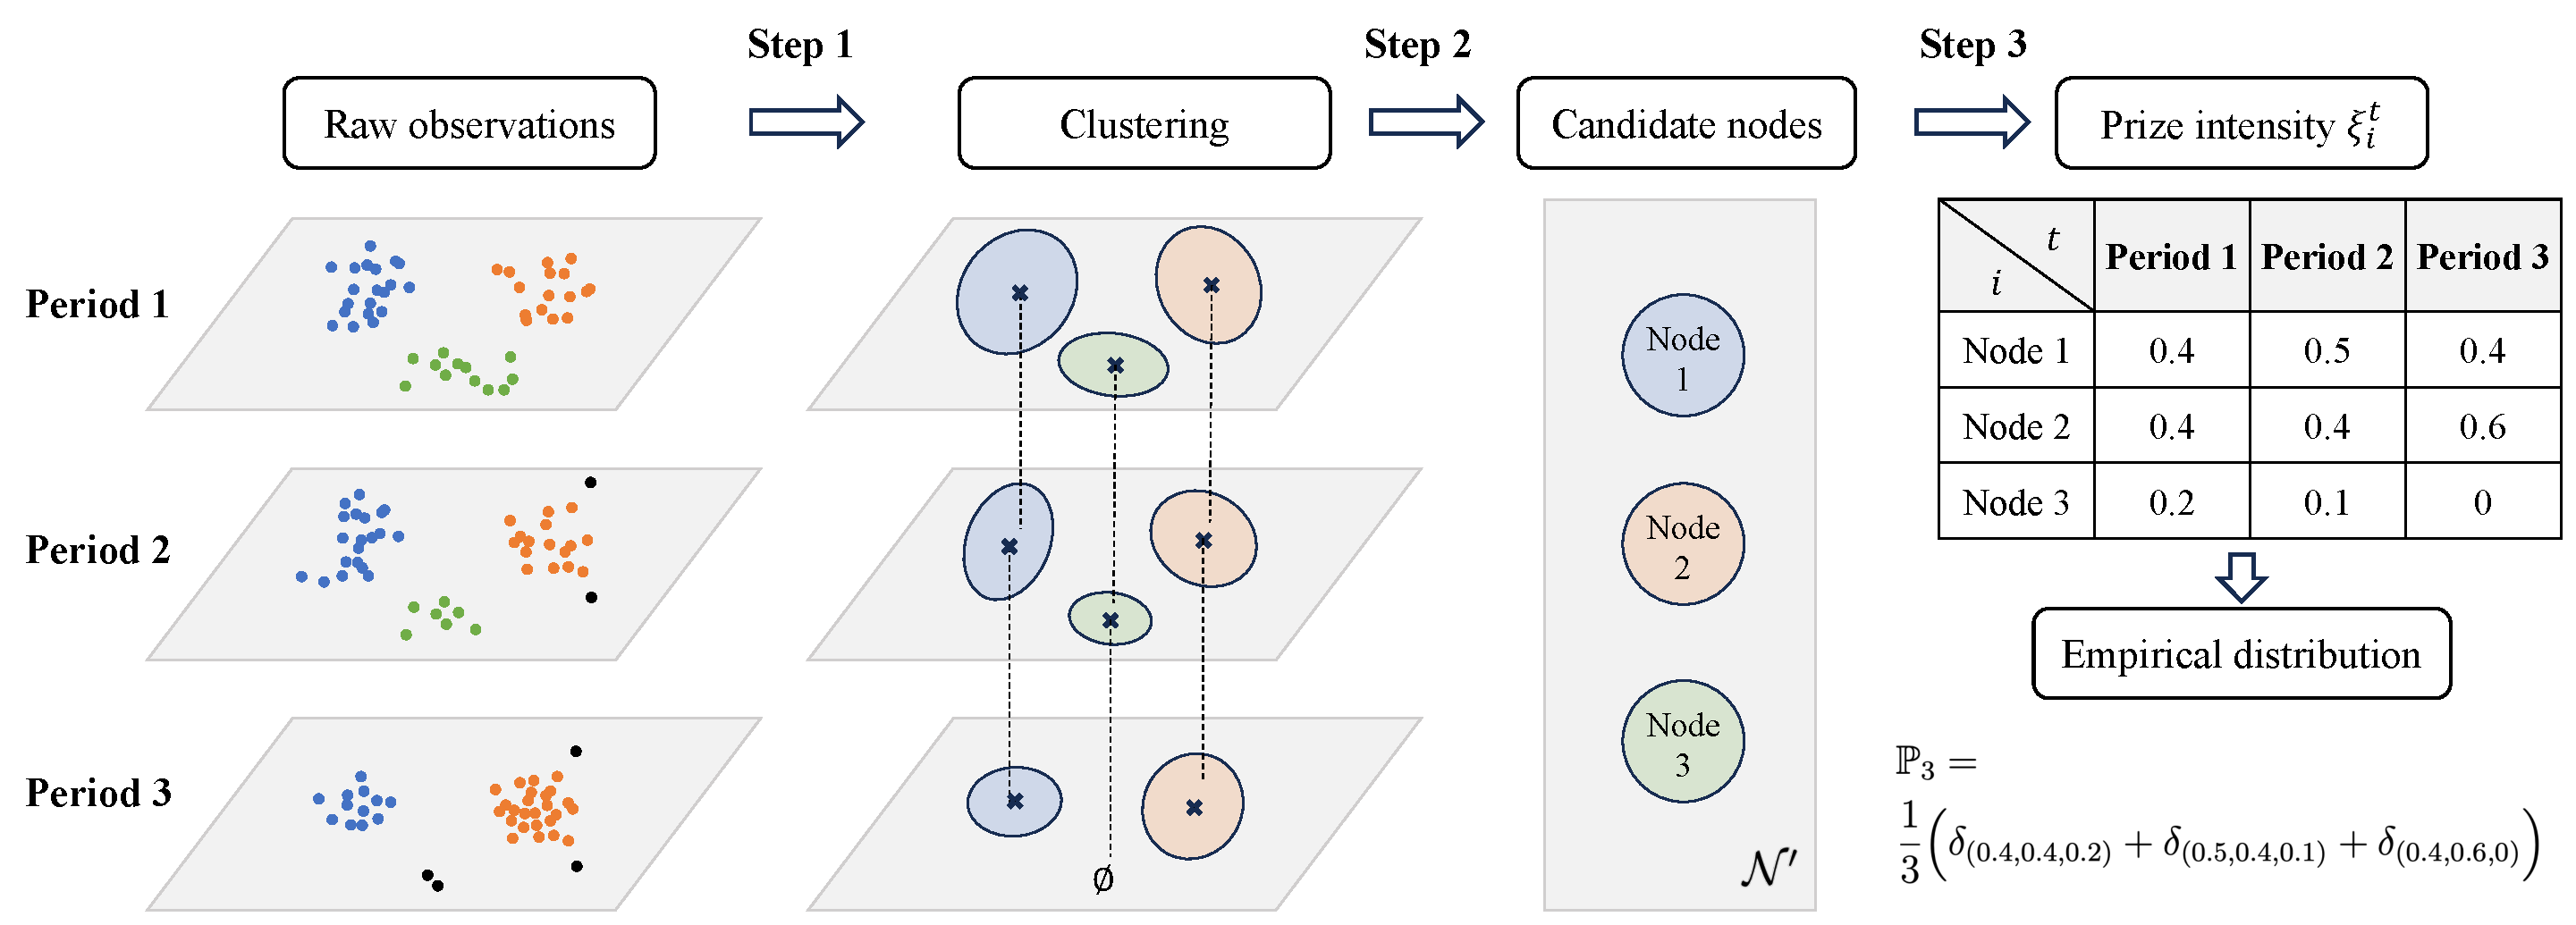
\includegraphics[width=1\linewidth]{Illustration.pdf}
    \caption{Illustration of the candidate node identification and prize variation across observation periods. In Step 1, clusters are formed in each period independently. If the spatial distance between cluster points across the $\mathcal{T}$ periods is below a predefined threshold, they are merged into the same static candidate node (Step 2). The data mapped to this single node over the $\mathcal{T}$ periods then constitute its empirical data for calculating dynamic prizes (Step 3).}
    \label{fig:prize_variation}
\end{figure}


 
The prize vectors $\boldsymbol{\xi}^t = (\xi_1^t, \dots, \xi_n^t)$ are therefore treated as empirical samples of the joint probability distribution of prizes across all candidate nodes. The empirical distribution is constructed as
\begin{equation}
\mathbb{P}_T = \frac{1}{T} \sum_{t=1}^{T} \delta_{\boldsymbol{\xi}^t},
\end{equation}
where $\delta_{\boldsymbol{\xi}^t}$ denotes the Dirac measure at $\boldsymbol{\xi}^t$, meaning that $\mathbb{P}_T$ is a discrete distribution placing probability mass $1/T$ on each observed realization  $\boldsymbol{\xi}^t$. It essentially acts as a discrete approximation of reality when the true underlying distribution is unobservable. Figure~\ref{fig:prize_variation} illustrates the workflow from raw observations to period-varying prizes for candidate nodes. 

To hedge against the estimation error inherent in finite-sample approximation, we employ the Wasserstein metric to construct the ambiguity set. Since each component of the prize vector is obtained by period-wise normalization, the support set of the random prize vector is $\Xi=[0,1]^n$. We use the Euclidean ground metric $d(\boldsymbol{\xi},\boldsymbol{\zeta})=\|\boldsymbol{\xi}-\boldsymbol{\zeta}\|_2$ on $\Xi$. For two probability distributions $P$ and $Q$ supported on $\Xi$, the 1-Wasserstein distance is defined as
\begin{equation}
W(P,Q)=\inf_{\Pi\in\Gamma(P,Q)}
\int_{\Xi\times\Xi}
\|\boldsymbol{\xi}-\boldsymbol{\zeta}\|_2
d\Pi(\boldsymbol{\xi},\boldsymbol{\zeta}),
\label{eq:wasserstein_def}
\end{equation}
where $\Gamma(P,Q)$ is the set of all couplings with marginal distributions $P$ and $Q$. Accordingly, the Wasserstein ambiguity set is defined as:

\begin{equation}
\mathcal{P}_\epsilon = \{ \mathbb{P} : W(\mathbb{P}, \mathbb{P}_T) \le \epsilon \},
\end{equation}
\noindent containing all distributions within Wasserstein distance $\epsilon$ from $\mathbb{P}_T$, where $\epsilon$ is a tunable parameter that reflects the decision-maker's tolerance for distributional ambiguity.

With the candidate node set $\mathcal{N'}$ and the ambiguity set $\mathcal{P}_\epsilon$ established from the data-driven process, the routing optimization is formulated as follows. Define $\mathcal{N} = \{0\} \cup \mathcal{N'}$, where node $0$ denotes the depot. The directed arc set is $\mathcal{A}=\{(i,j)\in\mathcal{N}\times\mathcal{N}:i\neq j\}$, so self-loop variables are not defined. The travel cost matrix $C = [c_{ij}] \in \mathbb{R}^{(n+1)\times(n+1)}$ gives the cost from node $i$ to node $j$, and each vehicle is subject to a resource limit $U$. For each candidate node $i \in \mathcal{N'}$, let $\xi_i$ denote the random variable representing its prize, whose true distribution is unknown but lies within the ambiguity set $\mathcal{P}_\epsilon$; the empirical observations $\{\xi^t_i\}_{t=1}^\mathcal{T}$ defined above serve as finite samples of $\xi_i$.




Before stating the routing formulation, we make the following modeling assumptions explicit.

\textbf{Assumption 1 (Historical-period representativeness and joint dependence).}
The period-wise prize vectors $\{\boldsymbol{\xi}^t\}_{t=1}^{T}$ are treated as representative historical realizations of the random prize vector $\boldsymbol{\Xi}$ for the planning horizon. This assumption does not require independent node-wise prize realizations. Instead, the empirical distribution $\mathbb{P}_T$ is built from joint vector samples, so the joint distributional structure among nearby candidate nodes is retained. For example, if adjacent construction-waste truck clusters reflect the same underlying activity pattern, their prizes can rise or fall together within the same vector sample. Consequently, the Wasserstein ambiguity set is defined over joint distributions on $\Xi=[0,1]^n$, rather than over a product of independent marginal distributions. Routing decisions are therefore evaluated against joint missed-prize patterns, allowing the model to account for groups of correlated high-prize nodes instead of treating each node as statistically isolated.

\textbf{Assumption 2 (Static planning and deterministic execution).}
The route is planned for a fixed horizon. The empirical prize distribution is assumed to remain applicable during route execution, and new observations are used to update future planning periods rather than to dynamically revise the current route.

\textbf{Assumption 3 (Penalty-based prize-collecting objective).}
We adopt a penalty-based interpretation of the prize-collecting objective. If candidate node $i$ is not visited, the model incurs an uncertain missed-prize penalty $M\xi_i$; visiting the node avoids this penalty. In the environmental-management application, $M\xi_i$ represents the expected loss from missing a node with potential enforcement benefit, rather than an additional travel cost. For a fixed realization of $\boldsymbol{\xi}$, minimizing missed-prize penalties is equivalent to maximizing collected prizes up to a constant total prize, which is why the penalty form is used in the robust routing formulation.


\begin{remark}[Role of the penalty coefficient $M$]

The penalty coefficient $M$ is a substantive preference parameter that controls the trade-off between routing economy and the prize of visiting high-prize nodes. It is measured by routing-cost units per unit of normalized prize: if travel costs are $c$ units per kilometer, $M/c$ is the greatest additional distance that the objective assigns to avoiding one full unit of missed prize. When $M$ is small, the model prefers no route or selective coverage; when $M$ is large, missed-prize exposure dominates routing cost and the model approaches the broadest coverage allowed by the resource constraints. Since this choice can change the routing regime, $M$ is calibrated from decision outcomes rather than treated as a numerical big-M constant. Section~\ref{sec:m_calibration} presents a sensitivity analysis of routing decisions with respect to $M$.

\end{remark}

 





The complete mathematical formulation is as follows:

\begin{equation}
\min_{x,y,z} \max_{P \in \mathcal{P}_\epsilon} \left[ \sum_{k\in\mathcal{K}}\sum_{(i,j)\in\mathcal{A}} c_{ij}x_{ij}^k + \mathbb{E}_P \left[ \sum_{i=1}^{n} \xi_i M \left(1 - \sum_{k=1}^{K} y_i^k \right) \right] \right].
\label{equoj}
\end{equation}

\noindent Subject to the following constraints:

\begin{equation}
\sum_{j:(i,j)\in\mathcal{A}}x_{ij}^k=\sum_{j:(j,i)\in\mathcal{A}}x_{ji}^k=y_i^k, \quad \forall i \in \mathcal{N'}, k \in \mathcal{K},
\label{equ2}
\end{equation}

\begin{equation}
\sum_{j:(0,j)\in\mathcal{A}}x_{0j}^k=z_k, \quad \forall k \in \mathcal{K},
\label{equ3}
\end{equation}

\begin{equation}
\sum_{i:(i,0)\in\mathcal{A}}x_{i0}^k=z_k, \quad \forall k \in \mathcal{K},
\label{equ4}
\end{equation}

\begin{equation}
\sum_{k=1}^K y_i^k \leq 1, \quad \forall i \in \mathcal{N'},
\label{equ5}
\end{equation}

\begin{equation}
\sum_{(i,j)\in\mathcal{A}}c_{ij}x_{ij}^k\leq Uz_k, \quad \forall k \in \mathcal{K},
\label{equ6}
\end{equation}

\begin{equation}
u_i^k - u_j^k + n \cdot x_{ij}^k \leq n-1, \quad \forall (i,j)\in\mathcal{A}\cap(\mathcal{N}'\times\mathcal{N}'),\ k\in\mathcal{K},
\label{equ7}
\end{equation}

\begin{equation}
1 \leq u_i^k \leq n, \quad \forall i \in \mathcal{N'}, k \in \mathcal{K},
\label{equ8}
\end{equation}

\begin{equation}
\begin{aligned}
x_{ij}^k&\in\{0,1\}, &&\forall (i,j)\in\mathcal{A},\ k\in\mathcal{K},\\
y_i^k&\in\{0,1\}, &&\forall i\in\mathcal{N}',\ k\in\mathcal{K},\\
z_k&\in\{0,1\}, &&\forall k\in\mathcal{K}.
\end{aligned}
\label{equ9}
\end{equation} 

The objective \eqref{equoj} is to minimize the total cost under the worst-case probability distribution within the ambiguity set.  \eqref{equ2} articulates the flow balance constraints, ensuring that the total inflow into a node equals the total outflow. 
 \eqref{equ3} and \eqref{equ4} establish optional depot departure and return constraints through the vehicle-use variable $z_k$. Thus, not all vehicles must be used; if $z_k=0$, vehicle $k$ neither departs from nor returns to the depot, while if $z_k=1$, it forms one depot-rooted route.
 \eqref{equ5} stipulates that each candidate node may be visited by at most one vehicle. 
 \eqref{equ6} imposes a resource constraint only on used vehicles, ensuring that the total travel cost of vehicle $k$ does not exceed $U$ when $z_k=1$ and forcing zero travel when $z_k=0$.
\eqref{equ7} and \eqref{equ8} introduce subtour elimination constraints (Miller-Tucker-Zemlin), which prevent any subcycles from occurring in the vehicle routes through the use of auxiliary variable \(u_i^k\). 
Finally, \eqref{equ9} defines binary decision variables \(x_{ij}^k\), \(y_i^k\), and \(z_k\), where \(x_{ij}^k\) indicates whether vehicle \(k\) travels directly from node \(i\) to node \(j\), \(y_i^k\) indicates whether candidate node \(i\) is visited by vehicle \(k\), and \(z_k\) indicates whether vehicle $k$ is used. Since $x_{ij}^k$ is defined only for $(i,j)\in\mathcal{A}$, self-loops cannot represent node visits.
This problem is categorized as a distributionally robust optimization challenge, representing a robust extension of the PCVRP with stochastic parameters. Given its NP-hard nature, large-scale instances necessitate the design of efficient heuristic or approximation algorithms to derive satisfactory solutions. This formulation enables risk-aware yet cost-efficient routing by integrating probabilistic inference with constrained vehicle routing under distributional uncertainty.


\section{Solution framework}\label{sec4}


We propose a two-stage framework that integrates density-based clustering, uncertainty modeling, and distributionally robust routing. The algorithmic innovations are organized around three components, which are highlighted in the workflow in Figure~\ref{fig:model_architecture}. First, the AD-DBSCAN module adaptively adjusts the neighborhood radius, core threshold, and hash-function count to flexibly adjust search intensity in response to dynamically changing and spatially varying local densities, thereby enabling rapid computations while preserving clustering quality. Second, the uncertainty-modeling module converts cluster-size observations from different periods into empirical distribution and constructs the Wasserstein ambiguity set for the DR-PCVRP. Third, the POMO-NS module uses a reinforcement-learning policy as a structure-aware warm-start constructor before applying neighborhood search under a DRO-aware objective to refine routing and node selection decisions. In this way, the flowchart emphasizes not only the processing sequence, but also key innovations that connect observation-driven node construction, prize uncertainty characterization, and robust routing optimization.


\begin{figure*}[htbp]
    \centering
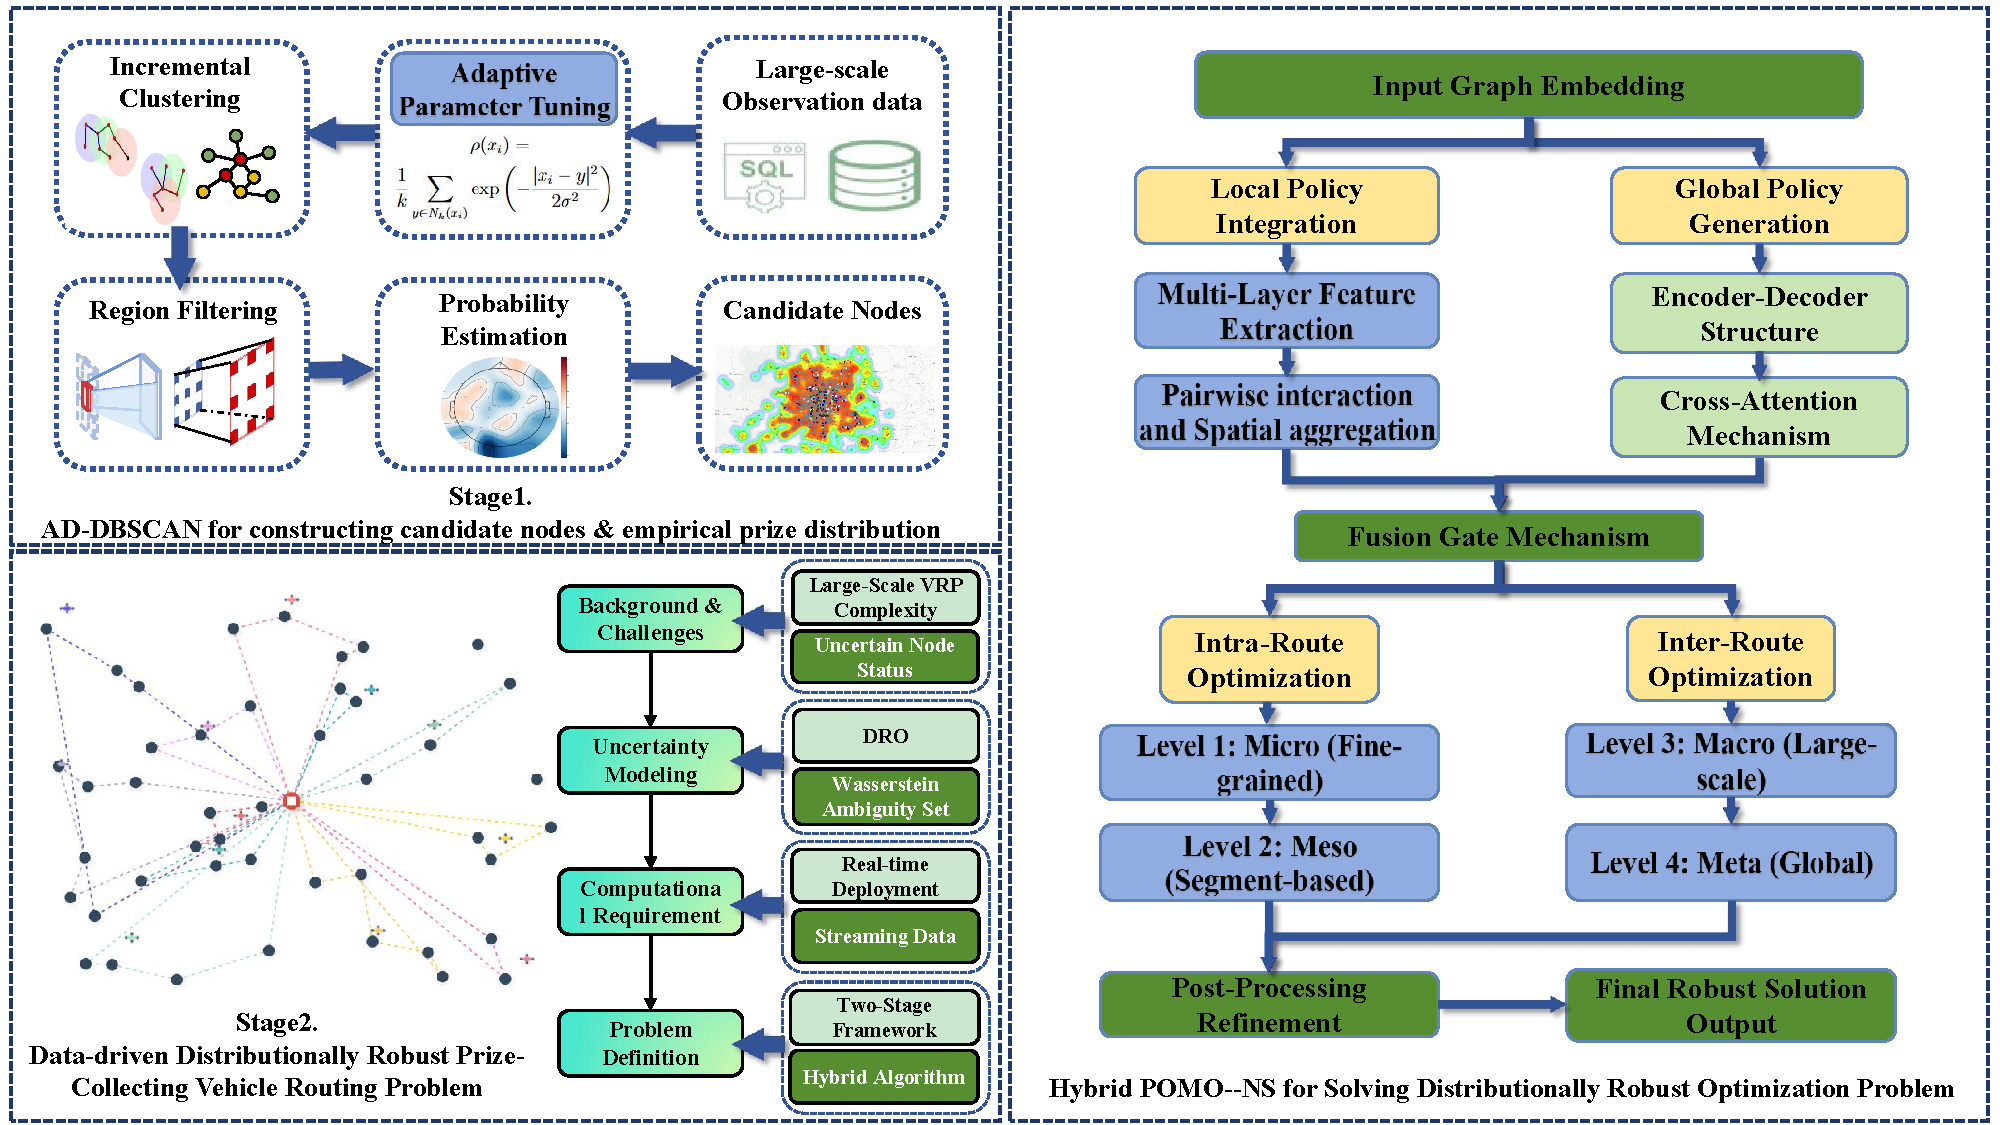
\includegraphics[width=\textwidth]{Graphical Abstract.pdf}
    \caption{Left: The complete model architecture consists of two main components: (1) candidate node identification using adaptive dynamic DBSCAN,  (2) problem modeling under distributional uncertainty. Right: The hybrid POMO-NS solution architecture for solving the DR-PCVRP. The innovative components of the proposed framework are shown as blue modules.}
\label{fig:model_architecture}
\end{figure*}



\subsection{Adaptive Dynamic DBSCAN to obtain the empirical distribution}
\label{sec:cluster}
\subsubsection{Overview of the AD-DBSCAN process}


In this work, to identify potential service locations and construct empirical distributions of their prizes, we adopt a density-based clustering approach, for the following reasons. First, locations or nodes requiring service often correspond to local high-density regions within the feature space, reflecting repeated or persistent patterns in historical or real-time observations.  Secondly, density-based clustering methods inherently accommodate clusters with varying shapes, sizes and densities, and do not necessitate a predefined cluster number, which are suited for modeling complex real-world data distributions. 



However, classical density-based methods, such as DBSCAN, encounter limitations when applied to large-scale datasets, due to their quadratic time complexity and inadequate scalability for streaming or dynamically growing data. These challenges become particularly critical in real-world applications where data records exceed millions. 
To address these issues, \citet{shin2025dynamic} propose a scalable alternative, namely dynamic DBSCAN, which extends classical DBSCAN by incorporating incremental updates and data-driven region modeling. Rather than recomputing global clusters with each change in data input, dynamic DBSCAN maintains a dynamic representation of the core point neighborhood graph, which enables the efficient addition of new data points while facilitating the removal of outdated records.


Relative to the Dynamic DBSCAN with Euler Tour Sequences framework of \citet{shin2025dynamic}, the methodological novelty of AD-DBSCAN lies in three adaptive parameter rules: the neighborhood radius $\varepsilon$, the core threshold $\kappa$, and the hash function count $r$. These three components are essential to the proposed algorithm because they determine, respectively, the local neighborhood scale, the density level required for core-point status, and the number of locality-sensitive hash projections used for neighborhood retrieval. By contrast, the sliding window, hash tables, and Euler tour tree are dynamic-maintenance primitives inherited from the original dynamic DBSCAN architecture. They are essential for streaming implementation and for preserving the polylogarithmic update structure, but they are not claimed as new algorithmic contributions. This distinction is important for the complexity analysis below: the adaptive parameters add a one-time and periodically amortized parameter-update cost, while the dynamic forest and hash structures determine the per-update clustering cost.

Throughout the AD-DBSCAN analysis, $m$ denotes the current clustering data size. In batch experiments, this equals the size of the dataset being clustered; in streaming applications, this equals the size of the current clustering window, not the cumulative number of historical observations received over time.



 
\subsubsection{Adaptive parameter formulation}
Classical dynamic DBSCAN algorithms rely on fixed hyperparameters (the neighborhood radius $\varepsilon$, core threshold $\kappa$, hash function count $r$), which restrict their adaptability to dynamic data streams characterized by non-uniform density distributions, concept drift, and variations in scale. To tackle these challenges, we propose the AD-DBSCAN algorithm, which dynamically adjusts the following critical parameters in response to the characteristics of streaming data.


\textbf{(1) Adaptive Neighborhood Radius $\varepsilon$:} For each point $x_i$, we compute the local density estimate:
\begin{equation}
\rho(x_i) = \frac{1}{\kappa} \sum_{y \in N_\kappa(x_i)} \exp\left(-\frac{|x_i - y|^2}{2\sigma^2}\right),
\label{e1}
\end{equation}
where $N_\kappa(x_i)$ denotes the nearest neighbors. The adaptive radius adjusts based on local density and data characteristics:
\begin{equation}
\varepsilon(x_i) = \varepsilon_0 \cdot \left(\frac{\bar{\rho}}{\rho(x_i)}\right)^{1/d},
\end{equation}
where $\bar{\rho}$ is the median density reference, and $d$ is the data dimension. This mechanism expands neighborhoods in sparse regions while contracting them in dense areas. 
For geospatial data (automatically detected when data are 2-dimensional and normalized), we apply specialized radius calculation:
\begin{equation}
\varepsilon_g = \bar{d} \cdot (c_1 - c_2 \cdot \log_{10}(\rho_s)) \cdot \left(1 + c_3 \cdot 
\log_{10}\left(\frac{m}{m_0}\right)\right),
\end{equation}
where $\bar{d}$ is the mean nearest neighbor distance and $\rho_s$ represents spatial density. For high-dimensional data, we apply dimensional adaptation to prevent the curse of dimensionality:
\begin{equation}
\varepsilon_d = \varepsilon_L + (\varepsilon_H - \varepsilon_L) \cdot \frac{1}{1 + \exp(-\gamma(d - d_0))},
\end{equation}
where $\varepsilon_L$ and $\varepsilon_H$ denote the lower and upper bounds of the radius range. The final radius is refined through multi-method optimization combining k-distance elbow detection, quantile-based estimation, and gradient analysis:
\begin{equation}
\varepsilon^* = \text{median}(\varepsilon_1, \varepsilon_2, \varepsilon_3),
\label{e2}
\end{equation}
where $\varepsilon_1, \varepsilon_2, \varepsilon_3$ represent the radius values suggested by the three methods respectively.

\vspace{.1 in}

\textbf{(2) Adaptive Core Threshold $\kappa$:} We compute the global dataset scale factor:
\begin{equation}
\delta = \log(m/m_0).
\label{e3}
\end{equation}
The core threshold is adjusted with data-type sensitivity parameter $\alpha$:
\begin{equation}
\kappa^* = \text{clip}(\lfloor \kappa_0 \cdot (1 + \alpha \cdot \delta) \rfloor, \kappa_L, \kappa_H),
\label{e4}
\end{equation}
\noindent where $\kappa_L$ and $\kappa_H$ are the minimum and maximum bounds. Under the definition of $m$ above, this rule scales the core point definition with the current clustering data size, preventing over-fragmentation in small datasets and over-aggregation in large datasets.
\vspace{.1 in}

\textbf{(3) Adaptive Hash Function Count $r$:} We scale the number of hash functions logarithmically with the current clustering data size $m$:
\begin{equation}
r^* = \left\lceil r_L + \beta \cdot \log_2\left(1 + \frac{m}{m_0}\right) \right\rceil,
\label{e5}
\end{equation}
where $r_L$ is the minimum hash function count. This balances computational efficiency with collision probability in the Locality-Sensitive Hashing structure, ensuring robust neighborhood queries as the active data volume grows.

These three adaptive mechanisms work synergistically: $\varepsilon$ adapts to local density patterns and data dimensionality, $\kappa$ scales with dataset size to maintain consistent cluster granularity, and $r$ adjusts the hash table complexity to preserve query efficiency. Together, they enable parameter-free clustering that automatically accommodates diverse data characteristics without manual tuning.

\subsubsection{Algorithmic architecture}

The AD-DBSCAN processes streaming data through an integrated sequence of operations. Its workflow consists of three phases: parameter initialization, dynamic clustering, and connectivity maintenance.

\textbf{Phase 1: Parameter Initialization.} The algorithm begins by computing the reference density $\bar{\rho}$ as the median density of the initial window of size $m_0$:

\begin{equation}    
\bar{\rho} = \underset{\bm{x}\,\text{in initial window}}{\text{median}} \left( \frac{1}{\kappa}\sum_{\bm{y} \in \mathcal{N}_\kappa(\bm{x})} \exp\left(-\frac{\|\bm{x} - \bm{y}\|^2}{2\sigma^2}\right) \right),
\end{equation}
based on data characteristics, the algorithm determines three adaptive parameters: the neighborhood radius $\varepsilon^*$ through Equations (\ref{e1}) - (\ref{e2}), the core threshold $\kappa^*$ through Equations (\ref{e3}) - (\ref{e4}), and the hash function count $r^*$ through Equation (\ref{e5}). The algorithm then constructs $r^*$ hash tables $\{\mathcal{H}_j\}_{j=1}^{r^*}$ and initializes the dynamic forest $\mathcal{F}$ for connectivity management.

\textbf{Phase 2: Dynamic Clustering.} For each arriving data point $\bm{x}$, the algorithm first updates the sliding window $W$ to retain only the most recent $h$ points through circular buffer management:

\begin{equation} 
W \leftarrow (W \cup \{\bm{x}\}) \setminus \{\bm{x}_{\text{oldest}}\} \quad \text{if} \quad |W| \geq m.
\end{equation}
\noindent An Euler-tree acceleration structure then enables efficient computation of the local density estimate $\rho(\bm{x})$, followed by determination of the point-adaptive neighborhood radius $\varepsilon(\bm{x})$, where $\varepsilon_L$ and $\varepsilon_H$ are the adaptive bounds determined during initialization.

The algorithm proceeds to calculate $r^*$ hash values using scale-adapted hash functions:

\begin{equation}
h_j(\bm{x}) = \left\lfloor \frac{\bm{x} + \eta_j \cdot \mathbf{1}_d}{2\varepsilon(\bm{x})} \right\rfloor, \quad \text{for} \quad j = 1,\dots,r^*,
\end{equation}
\noindent where $\eta_j$ are random offset vectors. Point $\bm{x}$ is added to corresponding buckets $\mathcal{H}_j[h_j(\bm{x})]$ and marked as a core point if any bucket satisfies the cardinality condition:
\begin{equation}
\exists j \in \{1,\dots,r^*\} ~\text{such that}~ \left|\mathcal{H}_j[h_j(\bm{x})]\right| \geq \kappa^*.
\end{equation}
\noindent At periodic intervals $\Delta\tau$, temporal adaptation activates through computation of the global density change rate:

\begin{equation}
\delta_\tau = \left| \frac{\rho_g(\tau) - \rho_g(\tau-\Delta \tau)}{\rho_g(\tau-\Delta \tau)} \right|,
\end{equation}
\noindent where $\rho_g(\tau)$ denotes the global density at time $\tau$. This triggers adjustment of the core threshold $\kappa^*(\tau)$  and hash function count $r^*(\tau)$, with hash tables dynamically resized while synchronizing the forest structure. Throughout processing, global density is maintained incrementally:

\begin{equation}
\rho_g(\tau) \leftarrow \frac{(m-1)\rho_g(\tau-1) + \rho(\bm{x})}{m}.
\end{equation}

\textbf{Phase 3: Connectivity Maintenance.}
The dynamic forest $\mathcal{F}$ continuously maintains connectivity: core points execute link operations $\mathcal{F}.\text{link}(\bm{x}, \bm{y})$ between all pairs sharing any bucket $(\exists j: h_j(\bm{x}) = h_j(\bm{y}))$, while non-core points connect via $\mathcal{F}.\text{link}(\bm{x}, \bm{y})$ to the first core point $\bm{y}$ satisfying $h_j(\bm{x}) = h_j(\bm{y})$ for some $j$. Euler Tour Tree operations ensure $O(\log m)$ connectivity management. Deletion operations mirror this workflow, removing points from buckets and forests while triggering a reevaluation of the core status for affected neighbors.

The complete algorithmic workflow, integrating adaptive parameter selection ($\varepsilon^*, \kappa^*, r^*$) with streaming data processing and dynamic connectivity maintenance, is formally presented in Algorithm \ref{alg:dynamicdbscan}.



\begin{algorithm}[htbp]
\caption{AD-DBSCAN}
\label{alg:dynamicdbscan}
\begin{algorithmic}[1]
\Require Initial window size $m_0$, parameters $(\varepsilon_0, \kappa_0, r_0)$, maximum sample size $s_{\max}$, window size $w$
\Ensure Filtered candidate set $\mathcal{V}_c = \{i \in \mathcal{I} \mid z_i = 1\}$

\State Set $m \leftarrow m_0$ and $s\leftarrow \min\{m_0,s_{\max}\}$
\State Compute $\bar{\rho} \leftarrow \operatorname{median}_{\bm{x}\,\text{in initial window}} \rho(\bm{x})$ where $\rho(\bm{x}) = \frac{1}{w}\sum_{\bm{y} \in \mathcal{N}_w(\bm{x})} \exp(-\|\bm{x} - \bm{y}\|^2/2\sigma^2)$
\State Detect dimension $d$ and geospatial flag
\State Compute $\varepsilon^*$ by Eqs.~(\ref{e1})--(\ref{e2}), $\kappa^* \leftarrow \text{clip}(\lfloor \kappa_0 (1 + \alpha \log(1+m/m_0)) \rfloor, \kappa_L, \kappa_H)$, $r^* \leftarrow \left\lceil r_L + \beta \log_2\left(1 + \frac{m}{m_0}\right) \right\rceil$
\State Initialize $\{\mathcal{H}_j\}_{j=1}^{r^*}$, $\mathcal{F}$, set $W$ to the initial window, $\rho_g \leftarrow \bar{\rho}$

\For{each arriving point $\bm{x}$}
    \State $m \leftarrow m + 1$; Update $W$; Compute $\rho(\bm{x})$, $\varepsilon(\bm{x}) \leftarrow \text{clip}(\varepsilon^* (\bar{\rho}/\rho(\bm{x}))^{1/d}, \varepsilon_L, \varepsilon_H)$
    \State \textbf{isCore} $\leftarrow$ False
    \For{$j = 1$ to $r^*$}
        \State $h_j(\bm{x}) \leftarrow \left\lfloor \dfrac{\bm{x} + \eta_j \mathbf{1}_d}{2\varepsilon(\bm{x})} \right\rfloor$; Insert $\bm{x}$ into $\mathcal{H}_j[h_j(\bm{x})]$
        \If{$|\mathcal{H}_j[h_j(\bm{x})]| \geq \kappa^*$}
            \State \textbf{isCore} $\leftarrow$ True
        \EndIf
    \EndFor
    \If{\textbf{isCore}}
        \State Link $\bm{x}$ to all $\bm{y}$ where $\exists j: h_j(\bm{x}) = h_j(\bm{y})$ via $\mathcal{F}.\text{link}(\bm{x}, \bm{y})$
    \Else
        \State Link $\bm{x}$ to the first core $\bm{y}$ with $h_j(\bm{x}) = h_j(\bm{y})$, if it exists
    \EndIf
    \State Assign $c(\bm{x})$ via $\mathcal{F}$; Update $\rho_g \leftarrow \dfrac{(m-1)\rho_g + \rho(\bm{x})}{m}$
    \If{$\tau \bmod \Delta\tau = 0$}
        \State $\delta_\tau \leftarrow \dfrac{|\rho_g(\tau) - \rho_g(\tau - \Delta\tau)|}{\rho_g(\tau - \Delta\tau)}$
        \State Update $\kappa^* \leftarrow \text{clip}(\lfloor \kappa_0 (1 + \alpha \delta_\tau) \rfloor, \kappa_L, \kappa_H)$
        \State Update $r^* \leftarrow \left\lceil r_L + \beta \log_2\left(1 + \dfrac{m}{m_0}\right) \right\rceil$; Resize $\{\mathcal{H}_j\}_{j=1}^{r^*}$
    \EndIf
\EndFor

\For{each region $i \in \mathcal{I}$}
    \State Compute $S_i, N_i, \bar{t}_i, C_i$; Set $z_i \leftarrow 1$
    \If{$N_i < N_{\min}$ or $\bar{t}_i \notin [t_{\min}, t_{\max}]$ or $C_i > C_{\text{thres}}$}
        \State $z_i \leftarrow 0$
    \EndIf
    \If{$z_i = 1$}
        \State $p_i \leftarrow S_i / N_i$
    \EndIf
\EndFor
\State \Return $\mathcal{V}_c = \{i \in \mathcal{I} \mid z_i = 1\}$
\end{algorithmic}
\end{algorithm}

\begin{theorem}[Amortized update complexity of AD-DBSCAN]\label{theorem2}

Using the above definition of $m$, let $d$ be the data dimension, $m_0$ the initial batch size, and $s=\min\{m_0,s_{\max}\}$ the sample size used for adaptive parameter estimation. Let $\varepsilon(\bm{x})$, $\kappa^*(m)$, and $r^*(m)$ denote the adaptive neighborhood radius, adaptive core threshold, and adaptive hash function count, respectively. Suppose the adaptive radius keeps the expected affected bucket size bounded by $B_{\varepsilon}(m)=O(\kappa^*(m))$, the adaptive rules satisfy $r^*(m)=O(\log m)$ and $\kappa^*(m)=O(\log m)$, and Euler tour tree link/cut/root operations take $O(\log m)$ time. After initialization, each insertion or deletion has expected amortized time
\[
O\!\left((r^*(m))^2\kappa^*(m)(d+\log m)+C_{\mathrm{adapt}}\right),
\]
where $C_{\mathrm{adapt}}$ is the cost of updating the adaptive parameters. The local density for $\varepsilon(\bm{x})$ is estimated from candidate neighbors returned by the hash-based index rather than from all points, so $C_{\mathrm{adapt}}=O(d\kappa^*(m))+O(C_{\mathrm{resize}}/\Delta\tau)$ under periodic adaptation. Under the stated adaptive rules, this becomes
\[
O(d\log^3 m+\log^4 m).
\]
For fixed-dimensional spatial data, this simplifies to $O(\log^4 m)$ after dropping lower-order dimension-dependent terms. The one-time initialization and adaptive parameter estimation cost is $O(s\log s+m_0 r^* d+m_0(r^*)^2\kappa^*(d+\log m_0))$ if the initial batch is inserted eagerly, while periodic resizing of hash tables is amortized over the streaming update horizon.


\end{theorem}
\begin{proof}
See Appendix A.
\end{proof}


Having established the AD-DBSCAN algorithm for identifying candidate nodes, we proceed to calculate the prize vectors $\boldsymbol{\xi}^t = (\xi_1^t, \dots, \xi_n^t)$, from which the empirical distribution $\mathbb{P}_T$ and the Wasserstein ambiguity set $\mathcal{P}_\epsilon$ are constructed and used as input for the second stage (see Section \ref{sec3}). 


\subsection{POMO-NS for solving distributionally robust PCVRP}
\label{POMO-NS}

We begin the second stage by clarifying the Wasserstein DRO term in \eqref{equoj}. The inner maximization problem reads (with the deterministic routing part omitted): 
\begin{equation}
\max_{P \in \mathcal{P}_{\epsilon}} 
\mathbb{E}_P \left[ 
\sum_{i=1}^n \xi_i \cdot M \cdot \left( 1 - \sum_{k=1}^K y_i^k \right) 
\right].
\label{10}
\end{equation}

For a fixed routing-and-selection decision $y$, define
\begin{equation}
f_y(\boldsymbol{\xi})=
\sum_{i=1}^n \xi_i M \left( 1 - \sum_{k=1}^K y_i^k \right),
\qquad \boldsymbol{\xi}\in\Xi=[0,1]^n .
\end{equation}
Under the Wasserstein distance defined in \eqref{eq:wasserstein_def}, the exact Kantorovich dual representation of \eqref{10} is
\begin{equation}
\sup_{P\in\mathcal{P}_\epsilon}\mathbb{E}_P[f_y(\boldsymbol{\xi})]
=
\inf_{\lambda\ge 0}
\left\{
\epsilon\lambda+
\frac{1}{T}\sum_{t=1}^{T}
\sup_{\boldsymbol{\xi}\in\Xi}
\left[
f_y(\boldsymbol{\xi})
-\lambda\|\boldsymbol{\xi}-\boldsymbol{\xi}^t\|_2
\right]
\right\}.
\label{11}
\end{equation}
Here $\lambda \geq 0$ is the dual variable associated with the Wasserstein radius, $\boldsymbol{\xi}^t$ is the $t$-th historical prize-vector sample, and the inner supremum explicitly allows each historical sample to be transported to a worst-case realization $\boldsymbol{\xi}\in[0,1]^n$. This expression is the standard exact dual form of the Wasserstein worst-case expectation.


{
\begin{proposition}[Exact finite-dimensional reformulation and candidate-solution evaluation]\label{prop:exact_reformulation}
For fixed $y$ and compact support $\Xi=[0,1]^n$, define
$a_i(y)=M\bigl(1-\sum_{k=1}^{K}y_i^k\bigr)$ for $i=1,\ldots,n$.
The worst-case expectation in \eqref{10}, equivalently represented by \eqref{11}, is the optimal value of the following SOCP:
\begin{equation}
\begin{aligned}
\phi_{\epsilon}(y)=
\min_{\lambda,\{\boldsymbol{q}^{t},\boldsymbol{s}^{t}\}_{t=1}^{T}}\quad
&\epsilon\lambda+
\frac{1}{T}\sum_{t=1}^{T}
\left[(\boldsymbol{q}^{t})^\top\boldsymbol{\xi}^t+
\boldsymbol{1}^\top\boldsymbol{s}^{t}\right]\\
\text{s.t.}\quad
&\|\boldsymbol{q}^{t}\|_2\leq\lambda,
&&t=1,\ldots,T,\\
&s_i^t\geq a_i(y)-q_i^t,
&&i=1,\ldots,n,\ t=1,\ldots,T,\\
&s_i^t\geq0,
&&i=1,\ldots,n,\ t=1,\ldots,T,\\
&\lambda\geq0,
\end{aligned}
\label{eq:exact_dro_socp}
\end{equation}
where $\boldsymbol{q}^{t}\in\mathbb{R}^{n}$ is an auxiliary dual vector and $\boldsymbol{s}^{t}\in\mathbb{R}_{+}^{n}$ is a nonnegative auxiliary vector representing the positive-part terms. Consequently, for any fixed complete feasible candidate solution $(x,y)$, its distributionally robust objective value can be evaluated exactly as
\begin{equation}
F_{\mathrm{DR}}(x,y)=
\sum_{k\in\mathcal{K}}\sum_{(i,j)\in\mathcal{A}}c_{ij}x_{ij}^k
+\phi_{\epsilon}(y).
\label{12}
\end{equation}
Together with constraints~\eqref{equ2}--\eqref{equ9}, minimizing \eqref{12} is equivalent to the original Wasserstein DRO formulation~\eqref{equoj}. For fixed $y$, \eqref{eq:exact_dro_socp} is an exact continuous SOCP; jointly optimizing the routing and conic variables yields an exact MISOCP.
\end{proposition}
\begin{proof}
See Appendix B.
\end{proof}

The reinforcement-learning policy first constructs feasible initial routes that serve as warm starts for neighborhood search. Starting from these initial solutions, the neighborhood search heuristically generates candidate routes by modifying the route order or the visited-node set. Each complete candidate route generated during this search is compared with the incumbent using the exact DRO objective in \eqref{12}.
}


\subsubsection{Integrating global and local optimality in POMO}


We now detail the two core components of POMO-NS and focus on the algorithmic innovations that distinguish it from a standard neural routing policy. The global component employs a Transformer-based POMO policy for rapid construction of high-quality candidate routes, while the local component introduces neighborhood-aware refinement and DRO-aware evaluation to improve solution precision. To improve readability, we retain the main computational logic and key formulas in the main text, and omit excessive implementation-level steps that do not affect the core algorithmic contribution.

\begin{proposition}[Amortized complexity advantage]\label{prop2}
Consider a sequence of $N_{\mathrm{ins}}$ instances of DR-PCVRP, each with $n$ candidate nodes. Let $C_{\mathrm{eval}}$ denote the cost of a single DRO objective evaluation, and let $C_{\mathrm{fwd}}$ denote the cost of a single forward pass of the pre-trained neural policy. A population-based metaheuristic with population size $P$ and $G$ generations requires $\Theta(N_{\mathrm{ins}} \cdot P \cdot G \cdot C_{\mathrm{eval}})$ total computation. In contrast, a pre-trained neural policy with one-time training cost $C_{\mathrm{train}}$ requires $C_{\mathrm{train}} + \Theta(N_{\mathrm{ins}} \cdot (C_{\mathrm{fwd}} + C_{\mathrm{eval}}))$ total computation. The amortized per-instance cost of the neural approach is therefore $O(C_{\mathrm{fwd}} + C_{\mathrm{eval}})$ as $N_{\mathrm{ins}} \to \infty$. In particular, when $C_{\mathrm{fwd}} = O(C_{\mathrm{eval}})$, the amortized per-instance cost reduces to $O(C_{\mathrm{eval}})$, yielding a $\Theta(P \cdot G)$ reduction relative to the metaheuristic approach.
\end{proposition}
\begin{proof}
See Appendix C.
\end{proof}

\paragraph{Global Policy Architecture}
The global policy adopts a Transformer-based encoder-decoder architecture following the POMO framework~\citep{kwon2020pomo}. Each node $i$ is represented by $\mathbf{x}_i = [\mathbf{x}_i^{\text{coord}}, d_i, p_i]$, where $p_i$ is the empirical mean prize estimated from the empirical distribution $\mathbb{P}_T$. The encoder captures global structural dependencies through Multi-Head Attention (MHA):
\begin{equation}
\mathbf{h}_i^{(l)} = \text{MHA}\left(\mathbf{h}_i^{(l-1)}, \{\mathbf{h}_j^{(l-1)}\}_{j=1}^n\right),
\end{equation}
where $l$ indexes encoder layers and $n$ is the number of candidate nodes. At decoding step $t$, the compatibility between the context embedding $\mathbf{q}_t$ and node embedding $\mathbf{k}_i$ is computed as:
\begin{equation}
u_i^{\text{global}} = \frac{\mathbf{q}_t^{\top} \mathbf{k}_i}{\sqrt{d}}, \quad \forall i \in V_{\text{valid}},
\end{equation}
where $d$ is the embedding dimension and $\mathcal{V}_{\text{valid}}$ contains feasible nodes satisfying capacity and visit constraints.

\paragraph{Local Policy Design}
To strengthen generalization across different spatial distributions and problem scales, the local policy focuses on the $e$ nearest feasible neighbors $\mathcal{N}_e(f_t)$ of the current node $f_t$. The key design is to encode each neighbor $n_i \in \mathcal{N}_e(f_t)$ by relative local features:
\begin{equation}
\mathbf{x}_i^{\text{local}} = [\tilde{\rho}_i, \theta_i, \tilde{d}_i],
\quad
\tilde{\rho}_i = \frac{\rho_i}{\max\{\rho_j \mid n_j \in \mathcal{N}_e(f_t)\}},
\quad
\tilde{d}_i = \frac{d_i}{Q_{\text{remain}}},
\end{equation}
where $\rho_i$ and $\theta_i$ denote the relative distance and angle from the current node. This relative representation makes local patterns transferable and scale-insensitive~\citep{gao2023towards}. The local embedding is initialized as:
\begin{equation}
\mathbf{h}_i^{(0)} = \mathbf{W}^{(0)}\mathbf{x}_i^{\text{local}} + \mathbf{b}^{(0)} + \text{PE}(\mathbf{x}_i^{\text{local}}).
\end{equation}
To retain the main local-search innovation without overloading the text with implementation details, we summarize the local feature refinement by a graph-attention aggregation:
\begin{equation}
\mathbf{h}_i^{\text{loc}} = \mathbf{h}_i^{(0)} + \alpha_{\text{norm}} \sum_{j \in \mathcal{N}_e(f_t)} 
\text{softmax}_j\!\left(\mathbf{a}^{\top}[\mathbf{h}_i^{(0)} \| \mathbf{h}_j^{(0)}]\right)\mathbf{W}_v \mathbf{h}_j^{(0)},
\end{equation}
where $\mathbf{a}$ is a learned attention vector and $\|$ denotes concatenation. The local score is then computed through a bilinear scoring function:
\begin{equation}
u_i^{\text{local}} =
\frac{\mathbf{q}_t^{\top}\mathbf{W}_s\mathbf{h}_i^{\text{loc}}}{\sqrt{d_e}},
\quad \forall n_i \in \mathcal{N}_e(f_t),
\end{equation}
where $d_e$ is the local embedding dimension and $\mathbf{W}_s$ is a learned scoring matrix. This design preserves the fine-grained geometric information needed for local routing decisions while avoiding unnecessary architectural complexity in the main text.

\paragraph{Policy Fusion Mechanism}
The global and local policies are fused by first applying a normalized distance penalty to the global score:
\begin{equation}
\tilde{u}_i^{\text{global}} = \begin{cases}
u_i^{\text{global}} - \frac{\rho_i}{\max\{\rho_j \mid n_j \in \mathcal{N}_e(f_t)\}}, & \text{if } n_i \in \mathcal{N}_e(f_t), \\
u_i^{\text{global}} - \xi, & \text{otherwise},
\end{cases}
\end{equation}
where $\xi \geq 1$ penalizes non-neighbor nodes. The ensemble score is:
\begin{equation}
u_i^{\text{ens}} = \tilde{u}_i^{\text{global}} + u_i^{\text{local}}, \quad \forall i \in V_{\text{valid}}.
\end{equation}
After masking infeasible actions, the action probability is:
\begin{align}
\pi_{\text{ens}}(a_t \mid s_t) &= \text{softmax}(\mathbf{u}^{\text{masked}}), \\
\text{where } u_i^{\text{masked}} &= \begin{cases}
C \cdot \tanh(u_i^{\text{ens}}), & \text{if } n_i \in V_{\text{valid}}, \\
-\infty, & \text{otherwise}.
\end{cases}
\end{align}

\paragraph{Offline Training of the Warm-start Constructor}
The global and local neural policies are trained offline as a deterministic routing constructor. The training procedure keeps two essential stages: global-policy pretraining for initialization and joint training of the fused global-local policy. Following POMO, multiple rollouts are generated from different starting nodes, and the reward is the negative deterministic routing cost:
\begin{equation}
R(\tau) = -\text{Cost}_{\mathrm{VRP}}(\tau),
\end{equation}
where $\text{Cost}_{\mathrm{VRP}}(\cdot)$ evaluates travel cost and feasibility in the deterministic CVRP environment. Prize uncertainty is not included in this offline training objective. The gradient of the expected return $J(\tilde{\theta}, \theta)$ with respect to the global parameters $\tilde{\theta}$ and local parameters $\theta$ is estimated using REINFORCE with a shared POMO baseline:

\begin{equation}
\nabla_{\tilde{\theta}, \theta} J(\tilde{\theta}, \theta) = \frac{1}{NB} \sum_{i=1}^{B} \sum_{j=1}^{N} \left(R_{i,j} - \frac{1}{N} \sum_{j=1}^{N} R_{i,j}\right) \nabla_{\tilde{\theta}, \theta} \log \pi_{\text{ens}}(\tau_{i,j}),
\end{equation}
\noindent where $B$ is the batch size, $N$ is the number of rollouts, and $R_{i,j}$ is the reward of the $j$-th rollout on the $i$-th instance. At inference, the trained constructor provides initial route skeletons. These routes are then refined by MNS under the selected objective. For DR-PCVRP, each candidate neighbor is scored by
\begin{equation}
\text{Obj}_{\mathrm{DR}}(\tau)=\text{RoutingCost}(\tau)+\phi_{\epsilon}(y(\tau)),
\end{equation}
where $y(\tau)$ is the node-selection vector induced by route $\tau$ and $\phi_{\epsilon}$ is the exact Wasserstein worst-case penalty in \eqref{eq:exact_dro_socp}. Thus, exact DRO is incorporated through the inference-time evaluation and acceptance of neighborhood moves.

\paragraph{Data Augmentation}
To enhance generalization to unseen spatial layouts, we apply eight-fold data augmentation through rotations and reflections during inference and select the best solution among the augmented instances.

The simplified training and inference procedure is presented in Algorithm \ref{alg:pomo_training}, which retains the key algorithmic steps and highlights the innovation of combining global neural construction, local neighborhood scoring, and local-search refinement. Additional implementation details are provided in Appendix D.


\begin{algorithm}
\caption{POMO-NS Warm-start Training and DRO-aware Inference}
\label{alg:pomo_training}
\small
\begin{algorithmic}[1]
\Require Training set $m_{\text{train}}$, instance $I$, parameters $(T_1, T_2, N, B)$
\Ensure Optimized solution $\tau^*$
\State \textbf{Phase I: Global Policy Pretraining}
\For{batch $\{I_i\}_{i=1}^B \sim m_{\text{train}}$, epochs $1$ to $T_1$}
    \State Generate $\mathcal{T}$ trajectories $\{\tau_{i,j}\}$ via $\pi_{\text{global}}$ with distance penalty
    \State Compute deterministic routing rewards: $R_{i,j} = -\text{Cost}_{\mathrm{VRP}}(\tau_{i,j})$
    \State Update global policy using the POMO shared baseline
\EndFor
\State \textbf{Phase II: Joint Training with Local Neighborhood Policy}
\For{batch $\{I_i\}_{i=1}^B \sim m_{\text{train}}$, epochs $T_1$ to $T_2$}
    \For{each decoding step $t$}
        \State Compute global scores $\mathbf{u}^{\text{global}}$ via Transformer encoder
        \State Extract $\mathcal{N}_e(f_t)$ and compute relative local features $[\tilde{\rho}_i,\theta_i,\tilde{d}_i]$
        \State Compute local scores $\mathbf{u}^{\text{local}}$ by neighborhood attention
        \State Fuse global and local: $u_i^{\text{ens}} \leftarrow \tilde{u}_i^{\text{global}} + u_i^{\text{local}}$
        \State Sample action: $a_t \sim \pi_{\text{ens}}(u_i^{\text{ens}})$
    \EndFor
    \State Compute deterministic routing rewards: $R_{i,j} = -\text{Cost}_{\mathrm{VRP}}(\tau_{i,j})$
    \State Update both policies $(\tilde{\theta}, \theta)$ via policy gradient
\EndFor
\State \textbf{Phase III: DRO-aware Inference with Data Augmentation}
\State Generate eight augmented instances by rotations and reflections
\State Construct one warm-start route for each augmented instance using the trained policy
\State Refine each warm start by MNS under the selected objective
\If{DR-PCVRP is selected}
    \State Evaluate each complete neighbor by $\text{RoutingCost}(\tau)+\phi_{\epsilon}(y(\tau))$ using \eqref{eq:exact_dro_socp} and \eqref{12}
\Else
    \State Evaluate each neighbor by the corresponding VRP/SP/RO objective
\EndIf
\State \Return the best solution $\tau^*$
\end{algorithmic}
\end{algorithm}



\begin{proposition}[POMO-NS inference complexity]\label{prop3}
The per-instance inference complexity of the POMO-NS algorithm is
\[
O\!\left(n^{2} d + b\,\bar{r}^{\,2} n^{2}\right),
\]
where $d$ is the embedding dimension, $b$ is the number of routes in the constructed solution, and $\bar{r}$ is the average route length.
\end{proposition}

\begin{proof}
The inference complexity consists of two sequential phases.
First, the neural construction phase: the Transformer encoder performs $L$ layers of multi-head attention over $n$ nodes with embedding dimension $d$, each costing $O(n^2 d)$; the decoder autoregressively selects $O(n)$ nodes, each step involving attention over $O(n)$ candidates, yielding a total decoding cost of $O(n^2 d)$.
Second, the local search refinement phase: by Proposition~\ref{prop4}, each MNS iteration costs
$O\!\left(b\,\bar{r}^{\,2} n^{2}\right).$
Since $b\bar{r} \approx n$ in balanced solutions, the overall per-instance inference complexity is
$O\!\left(n^{2} d + b\,\bar{r}^{\,2} n^{2}\right).$
\end{proof}

\subsubsection{Multi-level neighborhood search algorithm}

To overcome the limitations of classical single-operator local search methods, which often suffer from premature convergence and limited exploration capability in complex solution spaces, we propose a Multi-Level Neighborhood Search (MNS) algorithm. 
This framework integrates multiple complementary neighborhood operators through an intelligent selection mechanism and explores the solution space at different granularities simultaneously. 
The algorithm organizes neighborhood operators into a four-level hierarchy based on their modification scope and computational complexity. 
Level 1 (Micro) performs single-node relocations within and between routes, providing fine-grained local refinement with minimal structural disruption. 
Level 2 (Meso) applies segment-based operations involving 2-3 consecutive nodes, including Or-opt moves and 2-opt edge exchanges, balancing exploration capability with computational efficiency. 
Level 3 (Macro) conducts large-scale segment exchanges and route restructuring involving 4$+$ nodes through cross-exchange and extended 3-opt procedures, facilitating escape from local optima. 
Level 4 (Meta) implements route-level reconstruction through ejection chains and string relocation mechanisms that propagate changes across multiple routes simultaneously, achieving global rebalancing of the solution structure.

The algorithm maintains a performance score for each operator and dynamically adjusts selection probabilities based on their historical effectiveness. Let $\Omega = \{\omega_1, \omega_2, \ldots, \omega_m\}$ denote the set of available operators. At each iteration ${t'}$, the selection probability for operator $\omega_i$ is computed via the softmax function with temperature parameter $\tau$:
\begin{equation}
P_{t'}(\omega_i) = \frac{\exp(Q_{t'}(\omega_i)/\tau)}{\sum_{j=1}^{m} \exp(Q_{t'}(\omega_j)/\tau)},
\end{equation}
where $Q_{t'}(\omega_i)$ represents the quality score of operator $\omega_i$ at iteration ${t'}$. The temperature parameter $\tau$ controls the exploration-exploitation trade-off, with higher values promoting uniform exploration and lower values favoring proven operators. The quality score is updated using an exponential moving average with learning rate $\gamma \in [0,1]$:
\begin{equation}
Q_{{t'}+1}(\omega_i) = \gamma \cdot Q_{t'}(\omega_i) + (1-\gamma) \cdot R_{t'}(\omega_i),
\end{equation}
where the reward $R_{t'}(\omega_i)$ quantifies the improvement achieved by operator $\omega_i$. Specifically, the reward is defined as $R_{t'}(\omega_i) = \frac{f(S_{t'}) - f(S_{{t'}+1})}{f(S^*) + \epsilon}$ when the operator produces an improvement, and $R_{t'}(\omega_i) = -\eta$ otherwise, where $f(S_{t'})$ denotes the objective value of solution $S_{t'}$, $S^*$ is the current best solution, $\epsilon$ is a small constant preventing division by zero, and $\eta$ is a penalty for non-improving moves.

To escape from deep local optima, the algorithm incorporates controlled perturbations when no improvement has been found for $\theta$ consecutive iterations. The perturbation intensity adapts dynamically to the depth of stagnation:
\begin{equation}
\text{Intensity}({t'}) = \min\left(\beta_{\text{base}} \cdot \left(1 + \log\left(\frac{t_{\text{stag}}}{\theta}\right)\right), \beta_{\text{max}}\right),
\end{equation}
where $t_{\text{stag}}$ is the number of stagnant iterations, $\beta_{\text{base}}$ is the base intensity, and $\beta_{\text{max}}$ is the maximum allowed intensity. High-intensity perturbations apply multiple random moves from macro-level operators to drastically restructure the current solution and explore distant regions of the solution space. The complete MNS procedure integrates these components into a cohesive framework, alternating between intensification through composite operators and diversification through strategic perturbations, with the balance controlled by the adaptive operator selection mechanism. Algorithm~\ref{alg:MNS} presents the detailed implementation of the proposed approach.

\begin{algorithm}[t]
\caption{Multi-Level Neighborhood Search}
\label{alg:MNS}
\begin{algorithmic}[1]
\Require Initial solution $S$, operators $\Omega$, parameters $(\gamma, \tau, \theta)$
\Ensure Optimized solution $S^*$
\State \textbf{Init:} $S^* \leftarrow S$, $Q[\omega_i] \leftarrow 1.0$, $t_{\text{stag}} \leftarrow 0$
\While{${t'} < T_{\max}$} 
    \State Sample operator $\omega \sim P_t$ via quality scores
    \State Generate $\mathcal{N}$ from four levels based on $\omega$:
    \State \quad Micro: relocate single nodes within/between routes
    \State \quad Meso: Or-opt (segments $\ell \in \{1,2,3\}$) and 2-opt
    \State \quad Macro: cross-exchange and 3-opt (segments $\ell \leq 4$)
    \State \quad Meta (prob. $P_{\text{meta}}$): ejection chains, string relocation
    \State $S_{\text{new}} \leftarrow \arg\min_{s' \in \mathcal{N}} f(s')$
    \If{$f(S_{\text{new}}) < f(S)$}
        \State $S \leftarrow S_{\text{new}}$
        \If{$f(S) < f(S^*)$} $S^* \leftarrow S$, $t_{\text{stag}} \leftarrow 0$
        \EndIf
    \Else\ $t_{\text{stag}} \leftarrow t_{\text{stag}} + 1$
    \EndIf
    \State Update $Q[\omega]$ via exponential moving average
    \If{$t_{\text{stag}} \geq \theta$} Perturb $S$, reset $t_{\text{stag}}$
    \EndIf
\EndWhile
\State \Return $S^*$
\end{algorithmic}
\end{algorithm}

\begin{proposition}[MNS iteration complexity]\label{prop4}
The time complexity of a single iteration of the Multi-Level Neighborhood Search is
\[
O\!\left(b\,\bar{r}^{\,2} n^{2}\right).
\]
\end{proposition}

\begin{proof}
The complexity is dominated by the neighborhood generation phase. Micro-level moves evaluate
$O(n\bar{r})$ relocations per iteration. Meso-level operations, including Or-opt and 2-opt, consider
$O(\bar{r}^{\,2})$ moves per route, totaling $
O(b\,\bar{r}^{\,2}) $ across all routes. Macro-level cross-exchanges examine $O(b^{2}\bar{r}^{\,2})$ segment pairs between route pairs. Meta-level ejection chains with maximum length $L_{\max}$ require $O(b\,n\,L_{\max}\bar{r})$
evaluations, where $L_{\max}$ is typically a small constant. Since $b\bar{r} \approx n$ in balanced solutions, the overall complexity per iteration is
$O\!\left(b\,\bar{r}^{\,2} n^{2}\right).$
\end{proof}

After each optimization operation, the algorithm performs strict constraint checking to ensure solution feasibility:
\begin{equation}
\text{IsFeasible}(R, q, Q) = \begin{cases} 
\text{True} & \text{if } \sum_{i \in R} q_i \leq Q \\
\text{False} & \text{otherwise}
\end{cases},
\end{equation}
\noindent where $Q$ represents the vehicle capacity constraint. The route cost calculation formula is:
\begin{equation}
\text{Cost}(R) = D_{0,r_1} + \sum_{i=1}^{|R|-1} D_{r_i,r_{i+1}} + D_{r_{|R|},0},
\end{equation}
\noindent where $D_{i,j}$ represents the distance from node $i$ to node $j$, and node 0 represents the depot. The total solution cost is the sum of all route costs:
\begin{equation}
\text{TotalCost}(\mathcal{S}) = \sum_{R \in \mathcal{S}} \text{Cost}(R).
\end{equation}
The following proposition establishes that, for the DR-PCVRP, the POMO-NS algorithm achieves runtime reduction compared to classical pure heuristic algorithms while maintaining solution quality. 



The entire process of the POMO-NS Algorithm is illustrated in Algorithm \ref{al:total_model}.
\begin{algorithm}[t]
\caption{POMO-NS Algorithm}
\label{al:total_model}
\small
\begin{algorithmic}[1]
\Require VRP instance $\mathcal{G} = (\mathcal{V}, \mathbf{C})$, depot $n_0$, capacity $Q$, fleet $\mathcal{K}$, empirical distribution $\mathbb{P}_T$, Wasserstein radius $\epsilon$
\Ensure Distributionally robust solution $\mathcal{S}^* = \{R_1, R_2, \ldots, R_k\}$
\State \textbf{Phase 1: Neural Construction (Global Exploration)}
\State Initialize problem instance with node features $\mathbf{x}_i = [x_i^{\text{coord}}, d_i, p_i]$ for $i \in \mathcal{V}'$
\State Generate initial solution $\mathcal{S}_0$ using POMO-NS with 8-fold augmentation (Algorithm~\ref{alg:pomo_training})
\State \textbf{Phase 2: Local Search Refinement (Constraint-Aware Optimization)}
\State Evaluate the exact DRO objective $F_{\mathrm{DR}}(\mathcal{S}_0)$ using \eqref{eq:exact_dro_socp} and \eqref{12}
\State Apply Multi-Level Neighborhood Search to $\mathcal{S}_0$ (Algorithm~\ref{alg:MNS})
\State Obtain refined solution $\mathcal{S}^*$ with improved DRO objective value
\State \textbf{Phase 3: Feasibility Verification}
\For{each route $R_i \in \mathcal{S}^*$}    
    \State Verify resource constraint: $\sum_{(i,j) \in R_i} c_{ij} \leq U$
\EndFor
\State \Return Optimized distributionally robust solution $\mathcal{S}^*$
\end{algorithmic}
\end{algorithm}
\section{Numerical experiments and case studies}\label{sec5}

\subsection{Data sources}

To evaluate the effectiveness and transferability of the proposed methods, we conduct numerical experiments on standard datasets used to benchmark clustering and routing algorithms.  
\begin{itemize}
\item For the clustering task, we utilize widely recognized benchmarking datasets, including  Letter, MNIST, Fashion, KDDCup99, and Covertype, which encompass a diverse array of structural and statistical characteristics. The Letter dataset comprises character feature vectors derived from pixel-level statistics, providing a moderate-dimensional testbed with well-separated clusters. MNIST consists of grayscale images depicting handwritten digits, presenting significant challenges due to its high dimensionality and overlapping distributions. The Fashion dataset comprises 10 clothing categories and is widely adopted as a benchmark for evaluating clustering and representation learning algorithms in high-dimensional visual feature spaces. KDDCup99 represents a high-dimensional network intrusion dataset characterized by substantial noise and unbalanced distributions, serving as a rigorous stress test for density-based methods. The Covertype dataset includes cartographic variables derived from forest data, presenting a large-scale challenge with non-Gaussian distributions and varying densities to evaluate the algorithm's scalability. The heterogeneity of these datasets allows us to comprehensively evaluate the robustness, adaptability, and clustering accuracy of our adaptive dynamic density-based clustering algorithm across a range of real-world scenarios and synthetic conditions. Because these labeled benchmark datasets are not designed to represent spatial point streams, we additionally construct an application-aligned two-dimensional GPS dataset from Chengdu construction-waste-truck observations. In this dataset, raw longitude-latitude points serve as clustering features, while rule-based stay-point extraction and grid assignment provide multi-cluster reference labels, with label 0 denoting non-stay/noise points and positive labels denoting distinct stay-point clusters. This setting evaluates whether clustering methods can recover stop-point patterns relevant to candidate-node construction.

\item To benchmark the proposed POMO-NS routing algorithm, we utilize standard test datasets from the combinatorial optimization literature, specifically, CVRPLIB  \citep{uchoa2017new}, covering node scales ranging from 100 to 1000 nodes. These datasets are widely recognized for benchmarking routing algorithms across varying problem scales and constraints. The CVRPLIB datasets introduce capacity constraints that necessitate generating multiple feasible routes to meet delivery limits. 
By experimenting on instances of increasing complexity, we demonstrate that POMO-NS not only yields high-quality solutions but also exhibits robust scalability across different problem sizes. 


\item As a case study of the integrated solution approach, we consider a real-world application scenario in urban environmental management. In particular, GPS data collected from over 9,000 construction waste trucks (CWTs) in Chengdu, China, are treated as empirical indicators of earthwork activities that signal potential air pollution. In response to streaming GPS data of CWTs, a group of environmental inspectors set out to patrol the urban area, aiming to maximize coverage of high-risk pollution sites within limited routing capacity; see Figure \ref{fig:CR} for a visual presentation of the application scenario. The GPS data, dated from April 10 to April 18 2024, comprise approximately 100 million trajectory points. 
\end{itemize}

\subsection{Evaluation results and analyses}

Our evaluation is divided into two parts. The first part focuses on assessing the performance of the proposed AD-DBSCAN algorithm, verifying its clustering accuracy and computational efficiency in identifying candidate nodes from large-scale trajectory data. The second part evaluates the POMO-NS algorithm for solving the distributionally robust vehicle routing problem, examining solution quality, convergence speed, and scalability across varying problem complexities.

\subsubsection{Performance evaluation of the AD-DBSCAN algorithm}

Table~\ref{tab:clustering_methods} presents an overview of the clustering methods that are compared with the proposed AD-DBSCAN algorithm. We employ three primary performance indicators: Runtime, Adjusted Rand Index (ARI), and Normalized Mutual Information (NMI). Although the clustering procedure is unsupervised, benchmark datasets often provide reference labels that are used solely for performance evaluation. In this context, ARI measures the agreement between clustering assignments and reference labels based on pairwise sample relationships, adjusted for chance.  It is calculated as:
\begin{equation}
\label{eq:ari}
\text{ARI} = \frac{\sum_{i,j}\binom{n_{ij}}{2} - \left[\sum_i\binom{a_i}{2}\sum_j\binom{b_j}{2}\right] \big/ \binom{n}{2}}{\frac{1}{2}\left[\sum_i\binom{a_i}{2} + \sum_j\binom{b_j}{2}\right] - \left[\sum_i\binom{a_i}{2}\sum_j\binom{b_j}{2}\right] \big/ \binom{n}{2}}
\end{equation}
\noindent where $n_{ij}$ denotes the number of observations in both true class $i$ and predicted cluster $j$, $a_i$ and $b_j$ represent the marginal sums of the true class $i$ and predicted cluster $j$ respectively, and $n$ is the total number of observations.

The NMI quantifies the shared information between clustering assignments and reference labels, indicating the extent to which the identified clusters recover the latent structure in the data. It is calculated as:
\begin{equation}
\label{eq:nmi}
\text{NMI}(U,V) = \frac{2 \cdot I(U;V)}{H(U) + H(V)}
\end{equation}
where $U$ and $V$ denote the reference labels and the clustering assignments respectively, $I(U;V)$ is the mutual information between $U$ and $V$, and $H(\cdot)$ represents the entropy.


\begin{table}[H]
\centering
\caption{Benchmark clustering methods}
\begin{tabularx}{\linewidth}{lX}
\hline
\textbf{Method} & \textbf{Description} \\
\hline
\addlinespace
DynamicDBSCAN \citep{shin2025dynamic} & Baseline dynamic density-based clustering method \\
\addlinespace
Fdbscan Naive \citep{esfandiari2021almost} & Enhanced DBSCAN variant with dynamic parameter tuning for segmentation \\
\addlinespace
Fdbscan Noncore & Simplified EMZ with fixed core parameters to assess adaptability impact \\
\addlinespace
Sklearn Dynamic \citep{pedregosa2011scikit} & Classical DBSCAN implementation from the Scikit-learn library, widely used for density-based clustering tasks \\
\addlinespace
AD-DBSCAN (proposed) & Proposed model with adaptive neighborhood and density adjustment \\
\hline
\end{tabularx}
\label{tab:clustering_methods}
\end{table}

\begin{table}[H]
\caption{Experimental results for different clustering algorithms across different datasets. The first and second places are indicated by bold and underline, respectively; --- indicates that the result is unavailable or not reported under a comparable setting.}
\label{tab:experimental_results}
\centering
\small
\begin{tabularx}{\textwidth}{llXXXXX} 
\toprule 
\textbf{Dataset} & \textbf{Metric} & \textbf{Dynamic DBSCAN} & \textbf{Fdbscan Naive} & \textbf{Fdbscan Noncore} & \textbf{Sklearn Dynamic} & \textbf{AD-DBSCAN} \\ 
\midrule 
\multirow{3}{*}{\textbf{Letter}} & Time & 4.6540 & 7.0009 & \underline{4.2314} & \textbf{1.6219} & 4.6291 \\ 
& ARI & 0.0090 & \textbf{0.0153} & 0.0000 & 0.0021 & \underline{0.0153} \\ 
& NMI & 0.1956 & \textbf{0.2399} & 0.0000 & 0.1996 & \underline{0.2191} \\ 
\addlinespace 
\multirow{3}{*}{\textbf{MNIST}} & Time & \textbf{12.0008} & 49.2375 & 18.1443 & 51.4858 & \underline{13.6494} \\ 
& ARI & \underline{0.0463} & 0.0400 & 0.0239 & 0.0171 & \textbf{0.0477} \\ 
& NMI & \underline{0.2371} & 0.2152 & 0.1634 & 0.1377 & \textbf{0.2466} \\ 
\addlinespace 
\multirow{3}{*}{\textbf{Fashion}} & Time & \underline{18.0776} & 47.7176 & \textbf{17.7712} & 53.4038 & 19.5498 \\ 
& ARI & \underline{0.0536} & 0.0508 & 0.0093 & 0.0007 & \textbf{0.0556} \\ 
& NMI & 0.1396 & \textbf{0.2707} & 0.1340 & 0.0532 & \underline{0.1451} \\ 
%\addlinespace 
%\multirow{3}{*}{\textbf{Blobs}} & Time & \underline{22.8783} & 50.1209 & \textbf{12.7726} & 31.3624 & 23.4544 \\ 
%& ARI & \underline{0.7309} & 0.7269 & \textbf{0.9460} & 0.3550 & 0.7296 \\ 
%& NMI & \underline{0.9081} & 0.8996 & \textbf{0.9425} & 0.6848 & 0.9057 \\ 
\addlinespace 
\multirow{3}{*}{\textbf{KDDCup99}} & Time & \underline{1375.6804} & --- & --- & --- & \textbf{1327.1336} \\ 
& ARI & \underline{0.9140} & --- & --- & --- & \textbf{0.9145} \\ 
& NMI & \underline{0.8040} & --- & --- & --- & \textbf{0.8041} \\ 
\addlinespace 
\multirow{3}{*}{\textbf{Covertype}} & Time & \textbf{2158.9120} & --- & --- & --- & \underline{2378.3651} \\ 
& ARI & \underline{0.0516} & --- & --- & --- & \textbf{0.0517} \\ 
& NMI & \underline{0.1994} & --- & --- & --- & \textbf{0.1996} \\ 
\addlinespace
\multirow{3}{*}{\textbf{Chengdu GPS}} & Time & 20.9624 & \underline{19.8079} & 19.9840 & --- & \textbf{18.0652} \\
& ARI & \underline{-0.0338} & -0.0368 & -0.0378 & --- & \textbf{0.0156} \\
& NMI & 0.1055 & \underline{0.1259} & 0.1182 & --- & \textbf{0.3301} \\
\bottomrule 
\end{tabularx}
\end{table}

As illustrated in Table \ref{tab:experimental_results}, the AD-DBSCAN algorithm demonstrates consistent and competitive performance, ranking 1st or 2nd across datasets spanning diverse scales, dimensionalities, and complexities. In terms of clustering quality, it achieves the highest or near-highest ARI and NMI scores, indicating strong adaptability to both high-dimensional feature spaces (e.g., MNIST, Fashion) and large-scale data volumes (e.g., KDDCup99). The adaptive parameter mechanism enables the algorithm to automatically accommodate varying density distributions without manual tuning, which is particularly advantageous in scenarios where fixed-parameter methods suffer from over-segmentation or under-segmentation.
Regarding computational efficiency, while the adaptive mechanism introduces modest overhead on smaller datasets, this cost is offset by substantial efficiency gains as data scale increases. Notably, on KDDCup99 and Covertype datasets, only AD-DBSCAN and Dynamic DBSCAN remain computationally feasible, with AD-DBSCAN achieving slightly lower runtime in the reported experiments.

The labeled benchmark datasets above are useful for testing general clustering robustness, but they do not fully capture the spatial, streaming, and density-based nature of the proposed application. We therefore add a GPS-based validation using Chengdu construction-waste-truck observations. To make ARI and NMI computable in this spatial setting, we construct a two-dimensional regional dataset with 57,646 raw GPS points, where longitude and latitude are used as features and rule-based stay-point extraction provides multi-cluster reference labels. Label 0 denotes non-stay/noise points, and positive labels denote 105 distinct stay-point clusters in the selected region. As shown in Table~\ref{tab:experimental_results}, AD-DBSCAN obtains the best time, ARI, and NMI among the comparable dynamic density-based methods on this application-aligned dataset. We further report application-oriented indicators in Table~\ref{tab:gps_clustering_validation}, including the number of raw GPS points, spatial clusters, noise ratio, candidate nodes retained for routing, and streaming runtime.

\begin{table}[H]
\centering
\caption{Application-aligned spatial clustering validation on Chengdu GPS observations.}
\label{tab:gps_clustering_validation}
\begingroup
\small
\renewcommand{\arraystretch}{1.2}
\setlength{\tabcolsep}{4pt}
\resizebox{\textwidth}{!}{%
\begin{tabular}{lcccp{4.2cm}c}
\toprule
\textbf{Validation setting} 
& \textbf{GPS points} 
& \textbf{Spatial clusters} 
& \textbf{Noise ratio} 
& \textbf{Candidate nodes} 
& \textbf{Runtime} \\
\midrule
Nine hourly GPS windows 
& 122,394 
& 2,543 raw clusters 
& 64.65\% 
& 635 merged nodes; 123 high-priority nodes 
& -- \\
Streaming AD-DBSCAN run 
& 57,100 
& 2,840 clusters 
& 0.00\% 
& 98 nodes with at least 100 observations 
& 22.905 s \\
\bottomrule
\end{tabular}%
}
\endgroup
\end{table}

Table~\ref{tab:gps_clustering_validation} shows that the clustering stage performs the intended candidate-node construction function in the real application. Across nine hourly windows, 122,394 raw GPS observations are reduced to 635 spatially merged candidate nodes, among which 123 high-priority nodes containing at least 100 observations and are therefore suitable for subsequent routing. In the streaming AD-DBSCAN run, 57,100 GPS observations are processed in 22.905 seconds, with an average update time of 0.395 seconds per 1,000 inserted observations. These results complement the labeled benchmark experiments by validating the clustering procedure on realistic spatial point-process data where candidate-node construction is the main operational objective. The resulting candidate nodes and optimized routes under different values of $\epsilon$ are visualized in Figure~\ref{fig:chengdu_epsilon_routes}, while the route cost, missed-prize and coverage consequences of varying $M$ are summarized in Figure~\ref{fig:chengdu_m_pareto}.





\subsubsection{Comparative evaluation of POMO-NS optimization}

In this section, we compare the performance of the proposed POMO-NS framework with state-of-the-art benchmarks. Table~\ref{tab:routing_methods} provides an overview of these alternatives. Performance evaluation emphasizes solution quality, speed of convergence, and algorithm scalability across varying levels of problem complexity.

\begin{table*}[h]
\centering
\caption{Benchmark routing algorithms}
\label{tab:routing_methods}
\small
\renewcommand{\arraystretch}{1.12}
\begin{tabularx}{\textwidth}{@{}>{\raggedright\arraybackslash}p{3.2cm}X@{}}
\toprule
\textbf{Method} & \textbf{Description} \\
\midrule
HGS \citep{vidal2022hybrid} 
& Heuristic algorithm for combinatorial optimization problems, focusing on high-quality solutions. \\

CPLEX \citep{bixby2002solving} 
& A complete directed-arc CVRP mixed-integer programming formulation with MTZ load constraints, solved by IBM ILOG CPLEX under the same short time limits. \\

OR-Tools \citep{crainic1988or} 
& Google's open-source optimization toolkit providing constraint programming, linear programming, and routing solvers for operations research problems. \\

OR-Tools-Tabu 
& An OR-Tools routing configuration using a savings-based initial solution and tabu-search local improvement. \\

OR-Tools-SA 
& An OR-Tools routing configuration using a savings-based initial solution and simulated-annealing local improvement. \\

POMO \citep{kwon2020pomo} 
& Policy Optimization with Multiple Optima, which explores multiple optimal solutions in combinatorial optimization. \\

POMO-NS (proposed) 
& A hybrid framework that combines deep reinforcement learning for global policy generation with multi-level neighborhood search for constraint-aware local refinement. \\
\bottomrule
\end{tabularx}
\end{table*}


 

The experimental results are presented in Table~\ref{tab:vrp_comparison} and Figure~\ref{fig:vrp_convergence}, providing a comprehensive performance evaluation across nine node scale ranges from 100 to 1000 nodes. The performance indicator for these algorithms is the optimality gap from the optimal objective value, which is provided by the CVRPLIB dataset. For stochastic or randomized procedures, three runs are performed and the average gap is reported. Table~\ref{tab:vrp_comparison} retains the Part E benchmark gap values at the standard 2, 5, 8, and 10 second budgets and adds the new baselines under the same nominal time limits, whereas Figure~\ref{fig:vrp_convergence} shows the corresponding recorded convergence trajectories. We further include two relevant OR-Tools metaheuristic baselines, OR-Tools-Tabu and OR-Tools-SA, and a stricter exact-model reference, CPLEX. The CPLEX baseline solves a complete directed-arc CVRP-MTZ formulation under the same 2, 5, 8, and 10 second limits. Its time-point results are reported using a best-so-far incumbent convention, so the recorded gap is non-increasing as the time budget increases. CPLEX finds a feasible incumbent only for the 100--200-node group at 8 and 10 seconds, with a gap of 48.83\%; for the remaining scale--time cells, no feasible incumbent is found within the short time budget. This result indicates the difficulty of solving the complete arc-flow model under practical time limits and provides a conservative exact-model reference for the routing comparison. HGS is retained as a strong heuristic benchmark for small and medium instances; as shown below, it achieves the best gaps in several small and medium cases, while POMO-NS is mainly intended to provide fast learning-based warm starts with neighborhood refinement and broad coverage under tight time budgets. Based on these results, we highlight two key advantages of the proposed POMO-NS algorithm.

\begin{table}[H]
\caption{VRP algorithm performance comparison across all node scales at standard time limits (2s, 5s, 8s, 10s). Gap values are reported in percentages. Bold and underline indicate the best and second-best results, respectively; ``--'' indicates no data available or no feasible incumbent found at that time limit.}
\label{tab:vrp_comparison}
\centering
\begingroup
\resizebox{\textwidth}{!}{%
\small
\setlength{\tabcolsep}{3pt}
\renewcommand{\arraystretch}{1.15}
\begin{tabular}{@{}lcccccccccccc@{}}
\toprule
\multirow{3}{*}{\textbf{Method}} & \multicolumn{4}{c}{\textbf{Node 100-200}} & \multicolumn{4}{c}{\textbf{Node 200-300}} & \multicolumn{4}{c}{\textbf{Node 300-400}} \\
\cmidrule(lr){2-5} \cmidrule(lr){6-9} \cmidrule(lr){10-13}
& \multicolumn{4}{c}{\textbf{Gap (\%) at Time Limit}} & \multicolumn{4}{c}{\textbf{Gap (\%) at Time Limit}} & \multicolumn{4}{c}{\textbf{Gap (\%) at Time Limit}} \\
& \textbf{2s} & \textbf{5s} & \textbf{8s} & \textbf{10s} & \textbf{2s} & \textbf{5s} & \textbf{8s} & \textbf{10s} & \textbf{2s} & \textbf{5s} & \textbf{8s} & \textbf{10s} \\
\midrule
HGS & \textbf{0.84} & \textbf{0.57} & \textbf{0.33} & \textbf{0.25} & \textbf{3.71} & \textbf{2.75} & \textbf{2.13} & \textbf{2.12} & -- & \textbf{2.96} & \textbf{2.21} & \textbf{2.17} \\
OR-Tools & 8.94 & 8.71 & 8.59 & 8.59 & 17.25 & 15.86 & 15.06 & 14.79 & 40.06 & 32.45 & 32.45 & 32.45 \\
OR-Tools-Tabu & 7.30 & 6.63 & 6.30 & 6.18 & 12.90 & 12.33 & 12.33 & 12.33 & 19.39 & 17.21 & 17.13 & 14.40 \\
OR-Tools-SA & 7.17 & 7.17 & 7.17 & 7.17 & 12.90 & 12.51 & 12.49 & 12.49 & 19.39 & 17.30 & 17.30 & 17.30 \\
CPLEX & -- & -- & 48.83 & 48.83 & -- & -- & -- & -- & -- & -- & -- & -- \\
POMO & 4.39 & 4.39 & 4.39 & 4.39 & \underline{5.73} & 5.73 & 5.73 & 5.73 & \underline{7.32} & 7.32 & 7.32 & 7.32 \\
POMO-NS & \underline{3.72} & \underline{3.63} & \underline{3.63} & \underline{3.63} & 5.92 & \underline{5.69} & \underline{5.50} & \underline{5.49} & \textbf{6.11} & \underline{6.11} & \underline{6.11} & \underline{5.98} \\
\midrule
\multirow{3}{*}{\textbf{Method}} & \multicolumn{4}{c}{\textbf{Node 400-500}} & \multicolumn{4}{c}{\textbf{Node 500-600}} & \multicolumn{4}{c}{\textbf{Node 600-700}} \\
\cmidrule(lr){2-5} \cmidrule(lr){6-9} \cmidrule(lr){10-13}
& \multicolumn{4}{c}{\textbf{Gap (\%) at Time Limit}} & \multicolumn{4}{c}{\textbf{Gap (\%) at Time Limit}} & \multicolumn{4}{c}{\textbf{Gap (\%) at Time Limit}} \\
& \textbf{2s} & \textbf{5s} & \textbf{8s} & \textbf{10s} & \textbf{2s} & \textbf{5s} & \textbf{8s} & \textbf{10s} & \textbf{2s} & \textbf{5s} & \textbf{8s} & \textbf{10s} \\
\midrule
HGS & -- & -- & \textbf{2.10} & \textbf{2.10} & -- & -- & -- & -- & -- & -- & -- & -- \\
OR-Tools & -- & \underline{4.86} & 4.86 & 4.86 & -- & \textbf{3.69} & \textbf{3.19} & \textbf{3.11} & -- & -- & 29.19 & 28.98 \\
OR-Tools-Tabu & \textbf{7.27} & 5.80 & 5.77 & 5.77 & \textbf{5.01} & \underline{4.42} & \underline{4.42} & \underline{4.42} & \textbf{14.28} & \underline{10.59} & \underline{9.38} & \underline{9.18} \\
OR-Tools-SA & \underline{7.27} & 5.81 & 5.77 & 5.77 & \underline{5.01} & 4.42 & 4.42 & 4.42 & \underline{14.28} & 10.59 & 9.38 & 9.18 \\
CPLEX & -- & -- & -- & -- & -- & -- & -- & -- & -- & -- & -- & -- \\
POMO & -- & 5.10 & 5.10 & 5.10 & -- & 7.54 & 7.54 & 7.54 & -- & 10.59 & 10.59 & 10.59 \\
POMO-NS & -- & \textbf{3.87} & \underline{3.80} & \underline{3.79} & -- & 6.72 & 6.30 & 6.16 & -- & \textbf{8.50} & \textbf{7.79} & \textbf{7.74} \\
\midrule
\multirow{3}{*}{\textbf{Method}} & \multicolumn{4}{c}{\textbf{Node 700-800}} & \multicolumn{4}{c}{\textbf{Node 800-900}} & \multicolumn{4}{c}{\textbf{Node 900-1000}} \\
\cmidrule(lr){2-5} \cmidrule(lr){6-9} \cmidrule(lr){10-13}
& \multicolumn{4}{c}{\textbf{Gap (\%) at Time Limit}} & \multicolumn{4}{c}{\textbf{Gap (\%) at Time Limit}} & \multicolumn{4}{c}{\textbf{Gap (\%) at Time Limit}} \\
& \textbf{2s} & \textbf{5s} & \textbf{8s} & \textbf{10s} & \textbf{2s} & \textbf{5s} & \textbf{8s} & \textbf{10s} & \textbf{2s} & \textbf{5s} & \textbf{8s} & \textbf{10s} \\
\midrule
HGS & -- & -- & -- & -- & -- & -- & -- & -- & -- & -- & -- & -- \\
OR-Tools & -- & -- & 10.35 & 10.17 & -- & -- & -- & \underline{7.16} & -- & -- & -- & -- \\
OR-Tools-Tabu & \textbf{9.73} & 8.97 & 8.59 & 8.58 & \textbf{11.42} & 10.66 & 9.47 & 9.38 & -- & -- & -- & -- \\
OR-Tools-SA & \underline{9.73} & 8.96 & 8.59 & 8.58 & \underline{11.42} & 10.66 & 9.47 & 9.38 & -- & -- & -- & -- \\
CPLEX & -- & -- & -- & -- & -- & -- & -- & -- & -- & -- & -- & -- \\
POMO & -- & \underline{7.52} & \underline{7.52} & \underline{7.52} & -- & \underline{8.50} & \underline{8.50} & 8.50 & -- & -- & \underline{6.71} & \underline{6.71} \\
POMO-NS & -- & \textbf{6.50} & \textbf{6.32} & \textbf{6.31} & -- & \textbf{6.60} & \textbf{6.05} & \textbf{6.03} & -- & -- & \textbf{6.36} & \textbf{6.21} \\
\bottomrule
\end{tabular}%
}
\endgroup
\end{table}


To assess whether the observed improvements are systematic rather than isolated, we conduct paired Wilcoxon signed-rank tests over all scale--time cells in which both POMO-NS and the benchmark algorithm produce results. The null hypothesis is that POMO-NS does not reduce the optimality gap relative to the benchmark; the one-sided alternative is that the benchmark gap minus the POMO-NS gap is positive.

\begin{table}[H]
\centering
\caption{Paired statistical comparison under the same computational budget.}
\label{tab:vrp_statistical_tests}
\begingroup
\small
\resizebox{\textwidth}{!}{%
\begin{tabular}{lcccc}
\toprule
\textbf{Benchmark compared with POMO-NS} & \textbf{Paired cells} & \textbf{Mean gap reduction (pp)} & \textbf{Wins/losses} & \textbf{Wilcoxon $p$-value} \\
\midrule
POMO & 29 & 1.18 & 28/1 & $5.59\times10^{-9}$ \\
OR-Tools & 23 & 9.53 & 20/3 & $3.02\times10^{-5}$ \\
OR-Tools-Tabu & 27 & 3.92 & 24/3 & $1.88\times10^{-6}$ \\
OR-Tools-SA & 27 & 4.14 & 24/3 & $1.88\times10^{-6}$ \\
CPLEX & 2 & 45.20 & 2/0 & $2.50\times10^{-1}$ \\
\bottomrule
\end{tabular}
}
\endgroup
\end{table}



\textbf{Advantage 1: Rapid High-Quality Solutions for Large-Scale Instances.}
As shown in Tables~\ref{tab:vrp_comparison} and~\ref{tab:vrp_statistical_tests}, the expanded benchmark confirms that POMO-NS remains competitive after adding more relevant metaheuristic and exact-model baselines. HGS achieves the smallest gaps on several small and medium instances, but fails to return feasible solutions for many larger instances under short time limits. OR-Tools-Tabu and OR-Tools-SA improve over the default OR-Tools configuration in several cases, but they remain less stable on large-scale instances. CPLEX rarely returns a feasible incumbent within 10 seconds, which illustrates why complete MIP formulations are not suitable as full-scale short-time baselines. POMO-NS improves upon POMO in 28 of 29 paired scale--time cells through neighborhood refinement and significantly reduces the gap relative to the default OR-Tools, OR-Tools-Tabu, and OR-Tools-SA baselines over paired comparisons.


\textbf{Advantage 2: Neighborhood-Based Precision Enhancement with Minimal Time Investment.} Figure~\ref{fig:vrp_convergence} visualizes the corresponding gap trajectories, where POMO exhibits constant performance due to its single forward-pass inference, while POMO-NS shows progressive improvement through iterative neighborhood refinement. The OR-Tools metaheuristic variants generally require longer search time to refine their solutions, whereas POMO-NS obtains most of its gains within a short inference window. The most visible refinements of POMO-NS occur within the first 5--8 seconds. For example, at the 5-second budget, the 500--600, 600--700, and 800--900 cases exhibit 10.9\%, 19.7\%, and 22.4\% relative improvements over POMO, respectively. 



\begin{figure}[ht]
    \centering
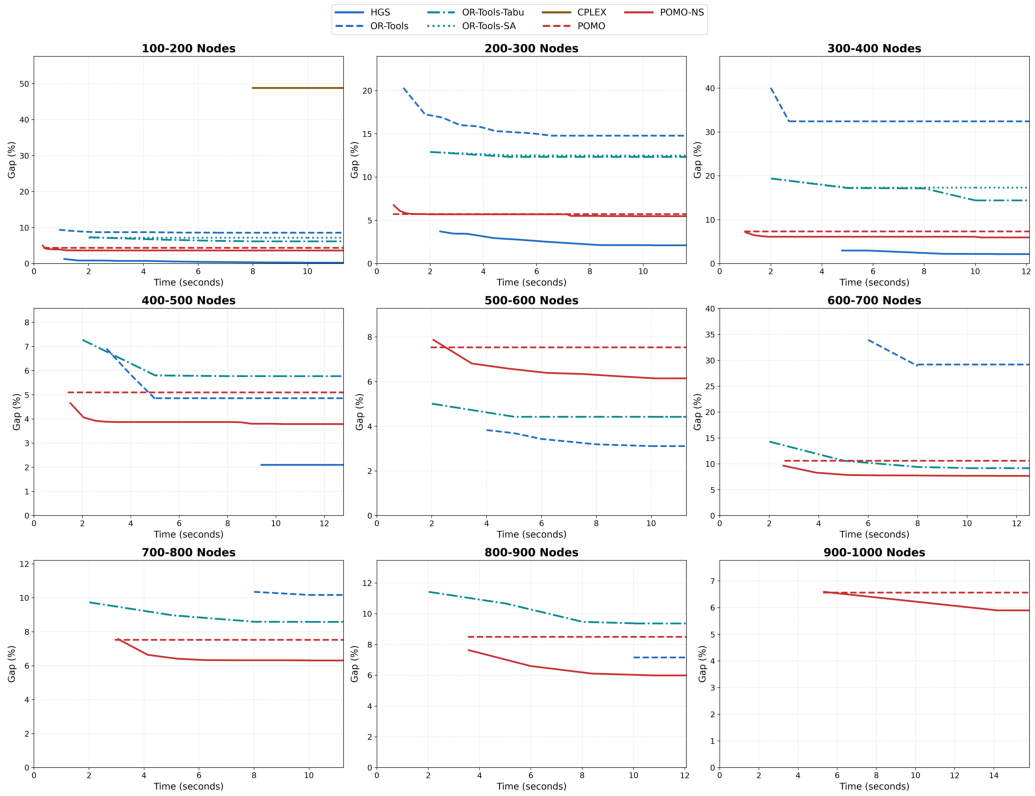
\includegraphics[width=\textwidth]{vrp_9_regions_mip_baselines.pdf}
    \caption{Performance comparison of VRP algorithms across different node scales and time limits. Each subplot corresponds to one of nine node scale ranges (100--200 to 900--1000 nodes) and displays the optimality gap (\%) as a function of the actual recorded computation time. The comparison includes HGS, OR-Tools, OR-Tools-Tabu, OR-Tools-SA, CPLEX, POMO, and the proposed POMO-NS. CPLEX denotes the complete directed-arc CVRP-MTZ formulation and appears only where a feasible incumbent is found within the time limit.}
\label{fig:vrp_convergence}
\end{figure}


The expanded experimental results provide more comprehensive validation for the design rationale of the hybrid algorithm. By leveraging POMO to generate high-quality initial solutions and using neighborhood search for refinement, POMO-NS improves the pure learning-based baseline while retaining short inference times. The added OR-Tools metaheuristic and CPLEX exact-model baseline further clarify the algorithmic trade-off: the complete arc-flow formulation rarely finds feasible incumbents under the same short time limits, whereas POMO-NS provides a lightweight learning-based warm start and local refinement mechanism that remains effective under limited inference time. Consequently, it provides a viable balance between performance and efficiency for practical large-scale VRP applications.

{
\subsubsection{Exact-DRO comparison and component ablation}
\label{sec:exact_dro_benchmark}

The preceding CVRPLIB experiment evaluates generic routing speed and scalability. 
However,  it does not test prize selection under distributional ambiguity. Therefore, we conduct a separate DR-PCVRP experiment in which every algorithm is optimized and compared under the exact Wasserstein objective $F_{\mathrm{DR}}$ in \eqref{12}. To keep this comparison consistent with the independent temporal validation, candidate locations and prize samples are constructed exclusively from the first seven days of the Chengdu data. This produces 250 fixed candidate locations and 168 hourly joint prize vectors from April 10--16, 2024, each with probability $1/168$ in $\mathbb{P}_T$; the final 48 hours are not used in this experiment. For each tested size $n\in\{10,15,20,40,80,120\}$, three instances are sampled by stratifying the 250 nodes according to their empirical mean-prize quintiles, thereby retaining both low- and high-prize nodes. The baseline parameters are $\epsilon=0.10$, $M=10^5$, and routing-resource ratio $R=0.55$.

Four algorithms are tested under the same exact objective and five-second wall-clock budget. GRASP-VND uses randomized restricted-candidate construction followed by variable-neighborhood descent \citep{feo1995grasp}; ILS-VND repeatedly perturbs an incumbent and reapplies the same descent neighborhoods \citep{lourenco2010ils}; ALNS-PC adaptively selects prize-collecting removal and reinsertion operators \citep{ropke2006alns}; and POMO-NS combines the neural warm start with the proposed MNS. All algorithms may insert, remove, exchange and reorder nodes subject to the same route constraints. Every node-set-changing move is accepted using the exact value of \eqref{eq:exact_dro_socp}, and every algorithm uses the same exact-evaluation cache policy within each run. Three seeds are used for every algorithm-instance pair. The analytical fixed-selection evaluator was additionally checked against the direct continuous SOCP on 12 randomly generated selections, with a maximum absolute discrepancy of $2.46\times10^{-5}$.

For the tractable instances, we solve the complete MISOCP formed by \eqref{equ2}--\eqref{equ9} and \eqref{eq:exact_dro_socp} using IBM ILOG CPLEX 22.1.1 with one thread and a 60-second limit. 
Table~\ref{tab:exact_dro_certification} reports the exact optimum whenever proved; 
otherwise, it reports the CPLEX lower bound and the best feasible incumbent found by CPLEX or the four heuristics. 
The certified gap is $(\mathrm{UB}-\mathrm{LB})/\mathrm{UB}$. CPLEX proves all three 10-node instances. The larger 168-sample MISOCP reaches the time limit for the 15- and 20-node instances, for which the solver bounds and best feasible solutions yield certified gaps from 0.95\% to 53.29\%. These intervals are reported as certificates, rather than treating an unverified best-known solution as an optimum.

\begin{table*}[htbp]
\centering
\caption{Exact MISOCP solutions and certified bounds under the Wasserstein DRO objective. Objective values are in $\times10^3$.}
\label{tab:exact_dro_certification}
\footnotesize
\setlength{\tabcolsep}{4.5pt}
\begin{tabular}{@{}lcrrrrr@{}}
\toprule
Instance & Status & \shortstack{CPLEX\\incumbent} & \shortstack{Lower\\bound} & \shortstack{Best\\feasible} & \shortstack{Certified\\gap} & \shortstack{Time\\(s)} \\
\midrule
$n10$-1 & Optimal & 63.48 & 63.48 & 63.48 & 0.00\% & 12.07 \\
$n10$-2 & Optimal & 34.19 & 34.19 & 34.19 & 0.00\% & 0.32 \\
$n10$-3 & Optimal & 49.34 & 49.34 & 49.34 & 0.00\% & 7.90 \\
$n15$-1 & Time limit & 58.81 & 39.83 & 54.67 & 27.16\% & 60.14 \\
$n15$-2 & Time limit & 35.87 & 35.53 & 35.87 & 0.95\% & 60.07 \\
$n15$-3 & Time limit & 46.62 & 34.35 & 40.83 & 15.88\% & 60.16 \\
$n20$-1 & Time limit & 128.81 & 42.67 & 51.87 & 17.72\% & 60.09 \\
$n20$-2 & Time limit & 78.15 & 29.98 & 64.17 & 53.29\% & 60.10 \\
$n20$-3 & Time limit & 129.34 & 31.91 & 49.53 & 35.56\% & 60.07 \\
\bottomrule
\end{tabular}
\parbox{0.97\textwidth}{\footnotesize ``Best feasible'' is the best incumbent returned by CPLEX or any compared algorithm; the lower bound always comes from CPLEX.}
\end{table*}

Table~\ref{tab:exact_dro_heuristics} compares the four algorithms under the same exact robust objective. The classical algorithms recover the 10-node optima to the evaluator tolerance, while POMO-NS has a 2.79\% mean gap. ALNS-PC has the lowest mean objective at 15 nodes and GRASP-VND at 20 nodes. POMO-NS becomes strongest from 40 nodes onward, with particularly large advantages at 80 and 120 nodes. Across all 54 paired runs, POMO-NS reduces the exact objective relative to GRASP-VND, ILS-VND, and ALNS-PC by 24.86\%, 26.34\%, and 23.42\% on average, respectively. The corresponding one-sided paired Wilcoxon tests give $p=9.34\times10^{-5}$, $p=5.73\times10^{-6}$, and $p=6.09\times10^{-5}$. The scale-wise results therefore identify both the small-instance setting in which classical prize-collecting search is competitive and the medium-to-large regime in which the neural warm start becomes most valuable.

\begin{table*}[htbp]
\centering
\caption{Strong-heuristic comparison under the same exact Wasserstein DRO objective. Entries are mean $\pm$ standard deviation in $\times10^3$ over three instances and three seeds; lower is better.}
\label{tab:exact_dro_heuristics}
\small
\resizebox{\textwidth}{!}{%
\begin{tabular}{lrrrrrr}
\toprule
Algorithm & $n=10$ & $n=15$ & $n=20$ & $n=40$ & $n=80$ & $n=120$ \\
\midrule
GRASP-VND & $\mathbf{49.01\pm12.69}$ & $46.79\pm6.54$ & $\mathbf{55.63\pm6.67}$ & $87.59\pm8.68$ & $619.06\pm28.88$ & $1109.72\pm34.47$ \\
ILS-VND & $\mathbf{49.01\pm12.69}$ & $49.36\pm8.52$ & $57.15\pm6.36$ & $95.68\pm11.94$ & $560.82\pm4.03$ & $1009.40\pm24.10$ \\
ALNS-PC & $\mathbf{49.01\pm12.69}$ & $\mathbf{45.55\pm8.15}$ & $57.15\pm6.36$ & $85.53\pm9.60$ & $565.68\pm9.67$ & $1003.41\pm9.53$ \\
POMO-NS & $50.52\pm13.89$ & $46.32\pm9.16$ & $58.21\pm11.32$ & $\mathbf{81.11\pm7.06}$ & $\mathbf{177.77\pm36.31}$ & $\mathbf{263.99\pm35.08}$ \\
\bottomrule
\end{tabular}}
\end{table*}

To separate the value of the warm start from that of neighborhood refinement, Table~\ref{tab:exact_dro_ablation} reports four controlled variants on the 40-, 80-, and 120-node instances. Greedy-MNS replaces only the POMO warm start with an exact-objective greedy constructor while retaining the full MNS; POMO removes all post-construction search; POMO-2opt retains only route-order 2-opt; and POMO-NS uses the complete node-selection and route-order neighborhoods. Relative to Greedy-MNS, POMO-NS lowers the objective by 52.27\% on average and wins 24 of 27 paired runs ($p=1.04\times10^{-7}$), which isolates the contribution of the learned warm start. Relative to pure POMO, full MNS lowers the objective by 5.51\% and records 23 wins and four ties ($p=1.33\times10^{-5}$). POMO and POMO-2opt remain nearly identical, whereas POMO-NS lowers the objective by 5.45\% relative to POMO-2opt ($p=2.29\times10^{-6}$). Thus, the effective refinement comes primarily from the node insert/remove/exchange neighborhoods that alter both the selected prize set and the route structure, rather than from route-order polishing alone.

\begin{table*}[htbp]
\centering
\caption{Warm-start and neighborhood ablation under the exact DRO objective. Entries are mean objectives in $\times10^3$ over three instances and three seeds.}
\label{tab:exact_dro_ablation}
\small
\begin{tabular}{lrrrl}
\toprule
Variant & $n=40$ & $n=80$ & $n=120$ & Component retained \\
\midrule
Greedy-MNS & 97.45 & 563.24 & 1003.41 & Greedy start + full MNS \\
POMO & 90.05 & 192.64 & 265.13 & Neural construction only \\
POMO-2opt & 90.03 & 192.44 & 265.05 & Neural construction + route-order 2-opt \\
POMO-NS & \textbf{81.11} & \textbf{178.41} & \textbf{263.97} & Neural construction + full MNS \\
\bottomrule
\end{tabular}
\end{table*}

Finally, we isolate the effect of the robustness model while holding the POMO-NS outer algorithm, instances, and five-second budget fixed. Routes are optimized with $\epsilon_{\mathrm{opt}}\in\{0,0.025,0.05,0.10,0.15,0.20\}$, after which every fixed route is reevaluated by the exact DRO evaluator at each $\epsilon_{\mathrm{eval}}$ in the same grid. The experiment uses ten 40-node instances, three seeds, $M=2.5\times10^4$, and $R=0.75$, so that routing cost and missed-prize exposure are simultaneously active. Table~\ref{tab:exact_dro_robustness_ablation} shows that entries within one evaluation-radius column use the same objective and are therefore directly comparable, whereas values across columns increase mechanically as the ambiguity set expands.  
Five of the six columns attain their lowest mean at the matching optimization radius: 
the only exception is $\epsilon_{\mathrm{eval}}=0.05$, for which the adjacent $\epsilon_{\mathrm{opt}}=0.025$ is slightly better. 
Under the baseline $\epsilon_{\mathrm{eval}}=0.10$, matching robust optimization lowers the mean exact objective from 43.407 to 42.986 relative to nominal optimization, a paired reduction of 0.91\% ($p=0.0087$), while increasing the visit rate from 84.08\% to 88.58\%. 
The benefit grows under stronger evaluation stress: the matched-radius reductions are 2.36\% at $\epsilon_{\mathrm{eval}}=0.15$ ($p=8.2\times10^{-5}$) and 4.29\% at $\epsilon_{\mathrm{eval}}=0.20$ ($p=2.0\times10^{-6}$). 
The matrix therefore shows that near-nominal routes remain competitive under mild distributional shifts, whereas robustly optimized routes become increasingly valuable as the admissible distributional deviation grows.

\begin{table*}[htbp]
\centering
\caption{Cross-evaluation of Wasserstein optimization and evaluation radii with the same POMO-NS outer search. Entries are mean exact objectives in $\times10^3$ over ten instances and three seeds; lower is better.}
\label{tab:exact_dro_robustness_ablation}
\small
\resizebox{\textwidth}{!}{%
\begin{tabular}{crrrrrrr}
\toprule
& \multicolumn{6}{c}{Evaluation radius $\epsilon_{\mathrm{eval}}$} & \\
\cmidrule(lr){2-7}
Optimization radius $\epsilon_{\mathrm{opt}}$ & 0.000 & 0.025 & 0.050 & 0.100 & 0.150 & 0.200 & Visit rate \\
\midrule
0.000 & \textbf{37.147} & 38.712 & 40.277 & 43.407 & 46.538 & 49.668 & 84.08\% \\
0.025 & 37.159 & \textbf{38.674} & \textbf{40.189} & 43.220 & 46.251 & 49.281 & 85.08\% \\
0.050 & 37.531 & 38.936 & 40.342 & 43.152 & 45.963 & 48.773 & 87.08\% \\
0.100 & 37.794 & 39.092 & 40.390 & \textbf{42.986} & 45.582 & 48.179 & 88.58\% \\
0.150 & 38.826 & 39.925 & 41.025 & 43.223 & \textbf{45.422} & 47.621 & 91.17\% \\
0.200 & 39.352 & 40.374 & 41.395 & 43.438 & 45.482 & \textbf{47.525} & 91.92\% \\
\bottomrule
\end{tabular}}
\parbox{0.97\textwidth}{\footnotesize Each row contains routes optimized at $\epsilon_{\mathrm{opt}}$; each column reevaluates those fixed routes at a common $\epsilon_{\mathrm{eval}}$. Bold entries are column minima. Comparisons are valid within, rather than across, evaluation-radius columns.}
\end{table*}
}



\subsection{Real-world case study}
To provide actionable real-world evidence, we apply the DR-PCVRP framework to the Chengdu trajectory dataset. 
First, we validate the constructed candidate locations. 
Then, the analysis evaluates fixed routing decisions through a chronological training--validation--test design.
Finally, we examine the decision sensitivity to $M$.

\subsubsection{External validation of candidate locations}
\label{sec:location_prize_validation}


The resulting clusters (candidate nodes) correspond to locations associated with different construction waste truck activities, including construction sites, quarry/concrete factories, parking lots, and dumping grounds \citep{yu2025using}. The process of extracting stay points from truck GPS trajectories, together with geo-referencing to the aforementioned points of interest (POIs), is reported in \citet{MA2026}. It should be noted that all these locations are potential sources of fugitive dust and particulate matter and are subject to environmental inspection and management. In fact, of all the 280 such clusters created in our computational instance, over 89.6\% have been previously visited by relevant personnel, based on the inspection record provided by the Chengdu Municipal Bureau of Ecological Environment. 

{






\subsubsection{Route-level temporal holdout validation}
\label{sec:temporal_holdout}

The preceding algorithmic experiments use resampled instances and therefore do not establish performance on genuinely unseen observation periods. Accordingly, we use a fixed chronological training--validation--test design for route-level model selection. A separate set of 250 candidate locations is frozen after hour 120 and held fixed while prize observations through hour 132 complete the training sample. Hours 1--132 form the training set, hours 133--168 form the validation set, and hours 169--216 form the independent test set. Hourly cluster counts are assigned to these fixed nodes and normalized within each hour. Following the holdout procedure in \citet{mohajerin2018data}, the route associated with the selected Wasserstein radius is retained directly after validation rather than refitted on the combined training and validation samples. No test observation is used to define candidate locations, select parameters, choose a start, or optimize a route.

We compare stochastic programming (SP), support-wide robust optimization (RO) and the exact Wasserstein DRO model with a strict chronological holdout. 
SP minimizes the empirical mean loss, whereas RO protects against every prize vector in $[0,1]^{250}$. For Exact DRO, $M=4000$ is fixed before calibration and $\epsilon$ is selected from $\{0.05,0.10,\ldots,0.50\}$ following the performance-driven holdout method of \citet{mohajerin2018data}. For each candidate radius, a route is optimized using only hours 1--132, fixed, and evaluated by its sample mean loss over hours 133--168; no Wasserstein ambiguity set is reconstructed on the validation sample. The validation mean is minimized at 68.777 ($\times10^3$) by $\epsilon=0.25$. The corresponding training route is retained without refitting and evaluated on hours 169--216. SP and RO are likewise optimized only on hours 1--132, after which all three fixed routes are evaluated by the same loss function on the independent test observations.

All three models use the same four-vehicle constraints, resource ratio $R=0.55$, coefficient $M=4000$, and POMO-NS search protocol. POMO generates 64 route candidates. Under each model's own training objective, duplicate visited-node sets are removed, the six best distinct feasible starts are retained, and each receives a three-second MNS refinement using the corresponding exact objective evaluator. Thus, the final routes are optimized separately rather than selected from a single fixed route pool, while the total neighborhood-search budget is identical across models. Each fixed route is evaluated in holdout hour $h$ by
\begin{equation}
C_h(y)=C_{\mathrm{route}}(y)+M\sum_{i=1}^{n}\xi_i^h\left(1-\sum_{k\in\mathcal{K}}y_i^k\right),
\qquad h=169,\ldots,216.
\label{eq:holdout_realized_cost}
\end{equation}
Uncertainty intervals are obtained from 10,000 circular moving-block bootstrap samples with four-hour blocks, preserving short-range temporal dependence.

\begin{table*}[htbp]
\centering
\caption{Kuhn-style independent temporal holdout results. Costs are in $\times10^3$; brackets contain 95\% moving-block bootstrap intervals.}
\label{tab:temporal_holdout}
\small
\resizebox{\textwidth}{!}{%
\begin{tabular}{lcccc}
\toprule
Model & Selected $\epsilon$ & \shortstack{Test performance\\$J_{\mathrm{test}}$ (95\% CI)} & \shortstack{Training estimate\\or certificate $\widehat J$} & \shortstack{Certificate margin\\$\widehat J-J_{\mathrm{test}}$} \\
\midrule
SP (SAA) & -- & 75.485 [74.630, 76.399] & 74.212$^{\dagger}$ & $-1.273$ \\
RO & -- & 74.733 [73.901, 75.651] & 281.432 & 206.698 \\
Exact DRO & 0.25 & \textbf{71.109} [69.097, 73.273] & 82.234 & 11.125 \\
\bottomrule
\end{tabular}}
\parbox{0.97\textwidth}{\footnotesize $J_{\mathrm{test}}$ is the sample mean out-of-sample loss over the 48 independent test hours. For Exact DRO and RO, $\widehat J$ is the corresponding training-period worst-case objective. $^{\dagger}$The SP entry is its training SAA estimate and is not a distributionally robust certificate. The certificate margin reports $\widehat J-J_{\mathrm{test}}$.}
\end{table*}

Exact DRO attains the lowest test performance and reduces mean out-of-sample loss by 4.376 and 3.625 relative to SP and RO, respectively (in $\times10^3$). 
It records a lower hourly loss in 41 of 48 comparisons against each baseline. 
The corresponding mean paired reductions have 95\% moving-block bootstrap intervals of $[2.747,5.801]$ and $[1.856,5.236]$; 
the two-sided Wilcoxon tests generate $p=4.75\times10^{-9}$ and $p=1.79\times10^{-7}$. 
The Exact-DRO certificate exceeds its independent test estimate by 11.125, whereas the SP training estimate falls 1.273 below its test performance. RO has a positive margin of 206.698, indicating a substantially less informative certificate. 
Thus, the Wasserstein model provides the best observed test performance together with a nonvacuous certificate in this temporal split.

To complement the statistical holdout results with the underlying spatial decisions, Figure~\ref{fig:chengdu_epsilon_routes} shows the routes optimized on the first 132 hourly prize vectors at six radii between $\epsilon=0.05$ and $0.50$. 
Every panel uses the same frozen 250-node set, four-vehicle constraints, route-resource ratio $R=0.55$ and $M=4000$. 
POMO supplies 64 candidates. 
After objective-specific pruning and visited-set deduplication, the six best distinct starts each receive a three-second MNS refinement using the exact inner DRO evaluator. 
The $\epsilon=0.25$ route, selected from the complete ten-radius grid by validation sample mean loss, is subsequently used without refitting in Table~\ref{tab:temporal_holdout}.

\begin{figure*}[htbp]
    \centering
    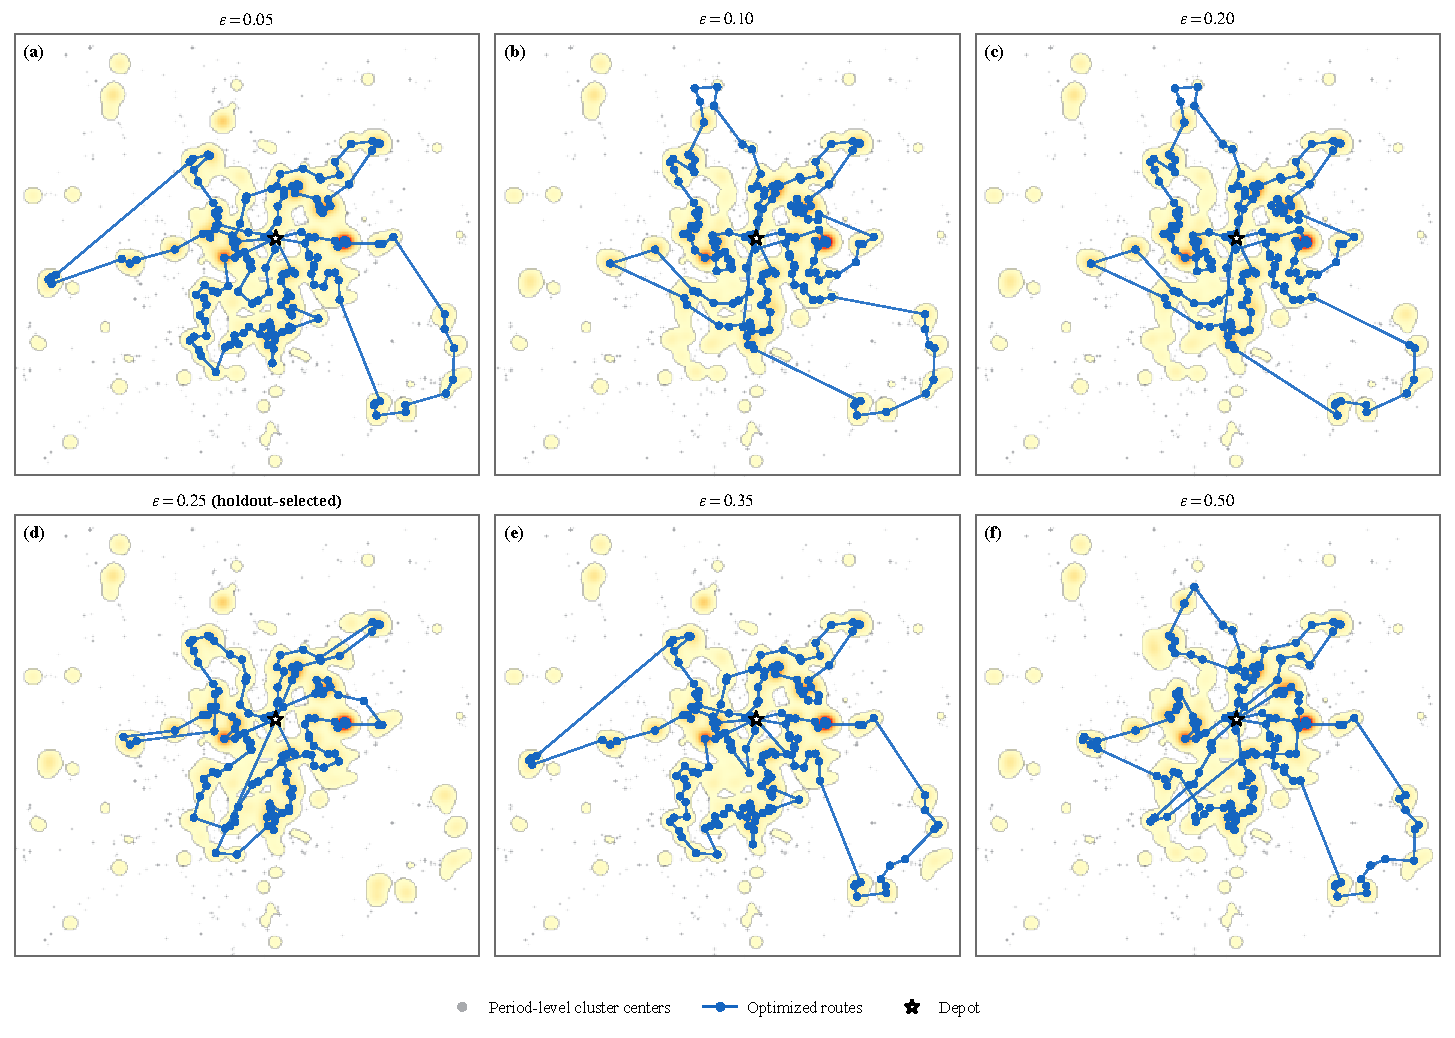
\includegraphics[width=\linewidth]{chengdu_routes_by_epsilon.pdf}
    \caption{Training-period route sensitivity to the Wasserstein radius $\epsilon$ in the Chengdu case study. Candidate nodes are fixed before validation, and the route models are fitted with hours 1--132 only and $M=4000$. The panels provide spatial illustrations of selected training decisions and are not holdout-performance metrics; each candidate objective uses the exact inner DRO evaluator.}
    \label{fig:chengdu_epsilon_routes}
\end{figure*}

\subsubsection{Conditional decision sensitivity of $M$}
\label{sec:m_calibration}

Since $M$ can alter the decision regime, we evaluate 33 policy-relevant levels from 0 to 100000 conditional on $\epsilon=0.10$. 
This experiment is a behavioral sensitivity analysis, not the joint calibration used in the route-level holdout comparison. 
To observe the complete transition from no deployment to full coverage, we use the relaxed route-resource ratio $R=1.0$, under which the four-route full-coverage reference is feasible; 
all other case-study comparisons retain their stated resource settings. 
The grid is refined around the empirically identified switching ranges, including six additional levels from 21000 to 25000. 
Travel costs are scaled at 100 units per kilometer, so $M/100$ is the distance-equivalent assigned to avoiding one full unit of missed prize. 
At each level, three distinct starts selected from the common POMO template pool and the feasible full-coverage reference receive separate 30-second MNS refinements. 
The experiment includes the full-coverage reference to ensure that a feasible zero-penalty regime cannot be hidden by warm-start failure. 
After all 99 runs, every distinct route is evaluated under every current value of $M$, and the lowest exact-DRO score defines the reported common candidate envelope. 
The empty route remains available at every level. 
Only the 168 training vectors enter route selection; the final 48 hours are used subsequently for descriptive holdout coverage. 
Table~\ref{tab:m_sensitivity} reports representative decisions, while Figure~\ref{fig:chengdu_m_pareto} reports the complete grid.

\begin{table*}[htbp]
\centering
\caption{Representative best-known decisions from the 33-level conditional sensitivity analysis of $M$ at $\epsilon=0.10$ and relaxed route-resource ratio $R=1.0$.}
\label{tab:m_sensitivity}
\small
\resizebox{\textwidth}{!}{%
\begin{tabular}{rrrrrrrrr}
\toprule
$M$ & Equivalent km & Vehicles & Nodes & Route cost ($\times10^3$) & Unit missed prize & Weighted penalty ($\times10^3$) & Training coverage & Holdout coverage \\
\midrule
0 & 0.0 & 0 & 0 & 0.000 & 23.361124 & 0.000 & 0.00\% & 0.00\% \\
2500 & 25.0 & 1 & 2 & 2.735 & 22.112008 & 55.280 & 5.81\% & 5.54\% \\
4000 & 40.0 & 4 & 232 & 82.368 & 1.050628 & 4.203 & 97.14\% & 97.01\% \\
12000 & 120.0 & 4 & 242 & 88.847 & 0.503841 & 6.046 & 98.99\% & 98.33\% \\
20000 & 200.0 & 4 & 242 & 88.847 & 0.503841 & 10.077 & 98.99\% & 98.33\% \\
21000 & 210.0 & 4 & 243 & 89.920 & 0.452644 & 9.506 & 99.14\% & 98.70\% \\
22500 & 225.0 & 4 & 243 & 89.920 & 0.452644 & 10.185 & 99.14\% & 98.70\% \\
23000 & 230.0 & 4 & 250 & 100.184 & 0.000000 & 0.000 & 100.00\% & 100.00\% \\
100000 & 1000.0 & 4 & 250 & 100.184 & 0.000000 & 0.000 & 100.00\% & 100.00\% \\
\bottomrule
\end{tabular}}
\end{table*}

The experiment comprises 99 independent 30-second searches. 
The common candidate envelope has six decision regimes, and its unit robust missed prize is nonincreasing in $M$, as required by the lower envelope of feasible affine route scores. 
Figure~\ref{fig:chengdu_m_pareto}(a) decomposes the best-known objective into routing cost and the weighted penalty $M g(y_M)$. 
Figure~\ref{fig:chengdu_m_pareto}(b) separately reports the unit robust missed prize $g(y_M)$ and training-period prize coverage. 
This distinction is important: 
$g(y_M)$ decreases stepwise to zero, whereas $M g(y_M)$ may rise within a fixed-route regime and drop discontinuously when the preferred route changes. The curves connect computed outcomes only; 
no spline, response-surface fit, or artificial smoothing is applied.

\begin{figure*}[!htbp]
    \centering
    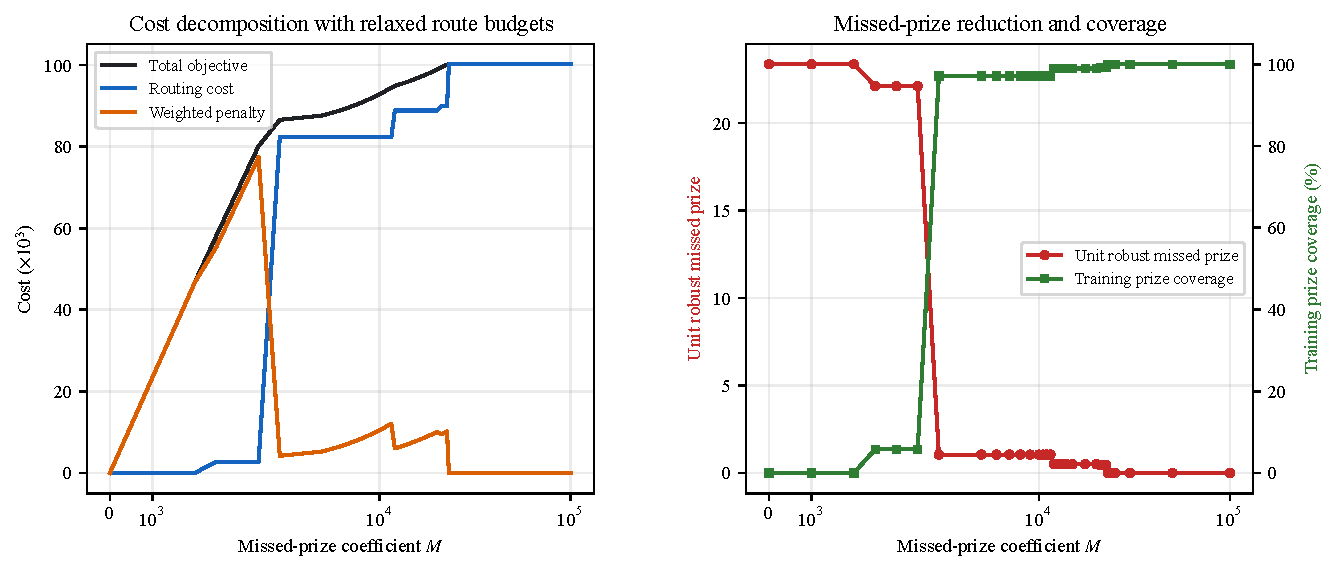
\includegraphics[width=0.96\linewidth]{M_sensitivity_relaxed_budget_R1_30s.pdf}
    \caption{Decision sensitivity to the missed-prize coefficient $M$ in the Chengdu case study, with $\epsilon=0.10$ and relaxed route-resource ratio $R=1.0$. Thirty-three levels are evaluated from 0 to 100000; three distinct starts receive 30-second MNS refinements at every level. Panel (a) decomposes the best-known objective into routing cost and weighted worst-case missed-prize penalty. Panel (b) shows the unit robust missed prize and training-period prize coverage. The feasible full-coverage reference is included in the common candidate pool.}
    \label{fig:chengdu_m_pareto}
\end{figure*}

The estimated intersections of consecutive affine route scores occur at $M\approx2189$, 3781, 11849, 20973 and 22676. 
On the evaluated grid, the empty route is followed by a two-node route at $M=2500$ and a broad-service four-vehicle route at $M=4000$, which visits 232 nodes and covers 97.14\% of the training prize. 
The preferred route visits 242 nodes from $M=12000$ and 243 nodes from $M=21000$. 
The final transition occurs between $M=22500$ and $M=23000$: above the estimated breakpoint $M\approx22676$, the 250-node full-coverage route is preferred, its routing cost is 100.184 ($\times10^3$), and both the unit and weighted missed-prize penalties equal zero. 
Thus, conditional on $\epsilon=0.10$ and $R=1.0$, the experiment reveals the complete behavioral range of $M$, from no deployment through selective and broad service to full coverage.
}




\clearpage
\section{Conclusion}\label{sec6}

This study develops and evaluates a data-driven DR-PCVRP framework for transforming massive observation data into robust selective-routing decisions. 
The main empirical findings are threefold. 
First, the proposed AD-DBSCAN procedure converts large-scale GPS observations into candidate inspection nodes and joint empirical prize-vector samples, making the downstream prize-collecting routing model operationally tractable. 
Second, under the same exact Wasserstein objective, the classical heuristics recover the certified 10-node optima to the evaluator tolerance, whereas POMO-NS obtains the best mean results from 40 to 120 nodes. 
The ablations show that the learned warm start and full neighborhood design reduce the objective by 52.27\% and 5.51\%, respectively, against their controlled counterparts. 
Third, the temporal holdout study evaluates out-of-sample routing performance.
Exact DRO obtains the lowest sample mean test loss, and its training certificate covers the independent test estimate with a substantially smaller margin than support-wide RO; 
the SP training estimate does not cover its test performance. 
Under a relaxed resource setting, conditional sensitivity at $\epsilon=0.10$ identifies the successive transitions from no route to selective, broad, and ultimately full coverage, where the missed-prize penalty becomes zero. Together, these results distinguish the contributions of the data-derived prize, robust model, learned warm start, neighborhood design and policy calibration.


\subsection{Theoretical implications}

This study develops an observation-driven implementation of distributionally robust prize-collecting routing by integrating candidate-node construction, joint prize-distribution estimation and robust route selection. 
To address computational infeasibility when potential locations exceed routing capacity, the framework uses density-based clustering to aggregate observation data into representative candidate nodes. 
This achieves strategic dimensionality reduction while preserving period-level dependence through joint empirical prize vectors. 
The revised formulation uses the exact finite-dimensional SOCP representation of the Wasserstein worst-case expectation for every fixed candidate solution, while the complete routing model is an exact MISOCP. 
The methodological contribution is a consistent data and solution interface across these components.


More specifically, the study contributes to the routing literature by endogenizing both candidate-node generation and prize uncertainty within a prize-collecting routing framework. 
Unlike conventional PCVRP models that assume a fixed set of nodes and deterministic prizes, the proposed formulation treats node importance as a random quantity learned from repeated observations. 
This modeling choice integrates data aggregation, ambiguity-set construction and routing decisions within one operational pipeline, and provides an observation-driven implementation of uncertainty-aware prize-collecting routing.


To process large-scale, dynamic observation data, we develop the AD-DBSCAN algorithm to efficiently identify candidate nodes and construct their empirical distributions. Utilizing a triple-adaptation mechanism for the neighborhood radius, core point thresholds, and hash function counts, the method handles non-uniform densities, concept drift, and scale variations. Under the stated hashing, bounded-bucket, and Euler-tour-tree assumptions, it achieves expected amortized $O(\log^4 m)$ per-update complexity for fixed-dimensional spatial data, improving scalability relative to classical DBSCAN recomputation under the stated update setting. Ultimately, by mitigating false positives via probabilistic filtering, it guarantees highly reliable input for the subsequent distributionally robust optimization model.

To efficiently solve the DR-PCVRP, we propose POMO-NS, a hybrid framework combining reinforcement learning with multi-level neighborhood search. The global Transformer-based component is used as a warm-start constructor that captures routing dependencies and local topological patterns learned from deterministic CVRP instances. The distributionally robust structure is then incorporated during inference through DRO-aware objective evaluation and neighborhood-search refinement. By separating fast route construction from risk-aware solution evaluation, this hybrid methodology provides a practical foundation for integrating deep reinforcement learning with classical operations research in large-scale prize-collecting routing problems.

\subsection{Practical implications}

In rapidly developing metropolitan regions, areas contaminated by construction waste pose significant threats to environmental safety and public health, creating urgent demands for more efficient monitoring and enforcement strategies. 
Our work was applied to Chengdu to convert observed truck activity into candidate inspection locations and exact-DRO routing priorities. 
The fixed chronological holdout design selects the Wasserstein radius by validation sample mean loss before evaluating fixed routes on the final two days, while the separate conditional $M$ experiment under relaxed route resources identifies the decision thresholds between no deployment, selective service, broad service and full coverage.


The results also provide several practical insights for agencies responsible for environmental patrol and urban freight governance. 
First, historical GPS trajectories can be used not only for retrospective analysis but also for forward-looking inspection planning: high-density and repeatedly observed truck activity can be converted into candidate nodes with uncertain but quantifiable priority. 
Second, $M$ represents the routing cost assigned to missed prize and should be calibrated with available route resources, as an increased $M$ shifts decisions from selective service toward broader coverage. 
Third, the chronological holdout separates parameter selection from final evaluation: 
Exact DRO attains the lowest sample mean test loss, its robust training objective covers the independent test estimate with a nonvacuous margin, and support-wide RO yields a much looser certificate. 
Therefore, decision makers should consider both out-of-sample performance and certificate informativeness when selecting the uncertainty model, $M$ and route-resource limit.

Emerging AI technologies can further enhance the usability of the proposed framework. Machine-learning components can continuously update candidate nodes and empirical prize distributions as new trajectory streams arrive, while generative AI interfaces can translate model outputs into human-readable patrol plans, risk explanations, and post-inspection summaries for decision makers. In this role, generative AI should be viewed as an interface and explanation layer built on top of the optimization model, rather than a replacement for the formal DR-PCVRP decision logic. Such human-in-the-loop integration can help environmental agencies move from static inspection schedules toward adaptive, explainable, and data-driven patrol systems.


\subsection{Limitations and future directions}

The independent evaluation is limited to one city; broader temporal and geographic validation is needed to establish transferability. The current framework addresses node identification and route optimization separately. Exploring tighter integration between the clustering stage and routing stage could potentially improve end-to-end performance.  For the AD-DBSCAN algorithm, although density-adaptive mechanisms enhance scalability, incorporating additional structural information and developing more sophisticated noise filtering strategies could improve clustering quality.  For the POMO-NS algorithm, while the combination of reinforcement learning and local search achieves strong performance, exploring advanced neural architectures and more diverse neighborhood operators could further enhance solution quality and generalization capability.  Future research can focus on more unified optimization frameworks that jointly optimize clustering and routing decisions, enhancing the adaptability of both algorithms to handle more complex problem structures. Moreover, extending the methodology to accommodate dynamic environments with real-time updates remains a promising future direction.

\section*{CRediT authorship contribution statement}
 

\section*{Declaration of competing interest}

The authors declare that they have no known competing financial interests or personal relationships that could have appeared to influence the work reported in this paper.

\section*{Acknowledgment}


\appendix
\section*{Appendix A. Proof of Theorem \ref{theorem2}}


\begin{proof}

We provide a more explicit derivation of the complexity of AD-DBSCAN and clarify the scope of the $O(\log^4 m)$ claim. The symbol $m$ follows the definition in Section~\ref{sec:cluster}: it is the current clustering data size. Let $d$ be the data dimension, $m_0$ the initial batch size, $s=\min\{m_0,s_{\max}\}$ the sample size used for adaptive parameter estimation, $\varepsilon(\bm{x})$ the adaptive radius, $r^*(m)$ the adaptive hash function count, $\kappa^*(m)$ the adaptive core threshold, and $C_{\mathrm{adapt}}$ the additional adaptive-parameter computation cost. The complexity statement refers to the expected amortized cost of one insertion or deletion after the dynamic structure has been initialized.

\paragraph{Role of the algorithmic components}
The three adaptive components introduced in AD-DBSCAN are $\varepsilon$, $\kappa$, and $r$. The adaptive radius $\varepsilon(\bm{x})$ controls the local neighborhood scale and reduces the risk of under-clustering sparse regions or over-clustering dense regions. The adaptive core threshold $\kappa^*$ controls the density level required for a point to become core. The adaptive hash function count $r^*$ controls the number of hash projections used for neighborhood retrieval and therefore affects the collision probability and candidate-bucket size. The sliding window, hash tables, and Euler tour tree are inherited dynamic-maintenance structures from Dynamic DBSCAN with Euler Tour Sequences; they are included in the complexity accounting, but they are not the new adaptive contribution of this paper.

\paragraph{Initialization and adaptive parameter estimation}
The adaptive parameters are estimated from an initial sample of size $s$. Computing the sampled $\kappa$-nearest-neighbor distances and the corresponding elbow/quantile statistics requires
\begin{equation}
T_{\varepsilon}=O(s\log s),
\end{equation}
when a standard indexed nearest-neighbor routine is used on the sampled set. The scale rule for $\kappa^*$ and the logarithmic rule for $r^*$ require only summary statistics and have lower-order cost. Initializing $r^*$ hash tables for $m_0$ points requires
\begin{equation}
T_{\mathrm{hash-init}}=O(m_0 r^* d),
\end{equation}
and initializing the dynamic forest requires at most linear node creation plus subsequent link operations generated by the hash buckets. If the initial batch is inserted eagerly into the dynamic connectivity structure, these bucket-induced link operations follow the same bound as the dynamic update operation applied to the $m_0$ initial points. Therefore, the initialization cost is written as
\begin{equation}
T_{\mathrm{init}}=O\!\left(s\log s+m_0 r^* d+m_0(r^*)^2\kappa^*(d+\log m_0)\right),
\end{equation}
which includes adaptive preprocessing, hash-table construction, and initial dynamic-forest connectivity. This term is a one-time cost and is not part of the per-update polylogarithmic claim. In long streaming applications, it is amortized over the number of subsequent insertions and deletions.

\paragraph{Single insertion or deletion}
For one arriving point, AD-DBSCAN first computes the adaptive quantities needed for local processing. The local density used for the adaptive radius is estimated from candidate neighbors retrieved by the hash-based index, rather than by scanning all active points. If the affected candidate set is bounded by the adaptive core threshold, this density computation costs
\begin{equation}
O(d\kappa^*(m)).
\end{equation}
This is the key condition under which the adaptive radius does not change the order of the update complexity; a global scan would instead require $O(md)$ and would invalidate the polylogarithmic per-update bound. Once $\varepsilon(\bm{x})$ is obtained, the algorithm computes $r^*(m)$ hash values and inserts or removes the point from the corresponding buckets, which costs $O(r^*(m)d)$.

The core-status check and candidate-neighbor retrieval are performed within the affected hash buckets. The adaptive radius $\varepsilon(\bm{x})$ determines the bucket width and thus the expected affected bucket size. We denote this bucket-size effect by $B_{\varepsilon}(m)$ and assume that the density-balancing radius rule keeps
\begin{equation}
B_{\varepsilon}(m)=O(\kappa^*(m)).
\end{equation}
Under this condition, neighborhood inspection over $r^*(m)$ hash projections is bounded by $O(r^*(m)\kappa^*(m))$ before dynamic connectivity updates.

The dynamic connectivity operations are handled by the Euler tour tree. Each link, cut, or root query takes $O(\log m)$ time. Following the dynamic DBSCAN analysis, an insertion or deletion may trigger interactions among affected buckets across pairs of hash projections, giving the parameterized update bound
\begin{equation}
T_{\mathrm{update}}
=O\!\left((r^*(m))^2\kappa^*(m)(d+\log m)+C_{\mathrm{adapt}}\right),
\label{eq:ad_complexity_general}
\end{equation}
where $C_{\mathrm{adapt}}$ collects the additional adaptive-parameter computation cost.
This expression includes local density estimation, adaptive radius computation, hash computation, candidate bucket inspection, core/non-core status updates, sliding-window insertion/deletion, and Euler-tour-tree link/cut operations. Cluster label queries after the update require $O(\log m)$ time and are dominated by $T_{\mathrm{update}}$.

\paragraph{Effect of the three adaptive parameters}
The three adaptive parameters enter \eqref{eq:ad_complexity_general} in different ways. First, $r^*(m)$ is the adaptive number of hash functions and appears as the squared hash-projection factor. If $r^*(m)$ were allowed to grow faster than logarithmically, the update complexity would increase accordingly. In our setting,
\begin{equation}
r^*(m)=O(\log m).
\end{equation}
Second, $\kappa^*(m)$ is the adaptive core threshold. Its numerical update is constant-time because it is computed from the current scale or density-change statistic. To avoid a full global reclassification, the updated threshold is applied to newly affected buckets and periodic maintenance operations rather than to all active points at every update. The rule satisfies
\begin{equation}
\kappa^*(m)=O(\log m),
\end{equation}
with practical clipping in the implementation. Third, $\varepsilon(\bm{x})$ affects the complexity indirectly: it controls the bucket width and candidate-neighbor size through $B_{\varepsilon}(m)$, while its local density estimate costs only $O(d\kappa^*(m))$ because candidate neighbors are retrieved from the hash-based index.

Therefore,
\begin{equation}
C_{\mathrm{adapt}}
=O(d\kappa^*(m))+O(C_{\mathrm{resize}}/\Delta\tau),
\end{equation}
where $C_{\mathrm{resize}}/\Delta\tau$ is the amortized cost of periodic hash-table resizing. Substituting $r^*(m)=O(\log m)$, $\kappa^*(m)=O(\log m)$, and $C_{\mathrm{adapt}}=O(d\log m)+O(C_{\mathrm{resize}}/\Delta\tau)$ into \eqref{eq:ad_complexity_general} yields
\begin{align}
T_{\mathrm{update}}
&=O\!\left((r^*(m))^2\kappa^*(m)(d+\log m)+C_{\mathrm{adapt}}\right) \\
&=O\!\left((\log m)^2(\log m)(d+\log m)+d\log m+\frac{C_{\mathrm{resize}}}{\Delta\tau}\right) \\
&=O\!\left(d\log^3 m+\log^4 m\right),
\end{align}
when periodic resizing is amortized over the streaming horizon. For fixed-dimensional geospatial data ($d=2$), the dimension-dependent term is lower order relative to $\log^4 m$, and the expected amortized per-update complexity is simplified to
\begin{equation}
T_{\mathrm{update}}=O(\log^4 m).
\end{equation}

\paragraph{Periodic adaptation and hash-table resizing}
The core threshold and hash function count are updated only at intervals of length $\Delta\tau$ or when the global density change exceeds the prescribed trigger. Full reclassification of all active points is not performed at every update. If resizing is required, the cost of rebuilding or synchronizing the affected hash tables is amortized over the updates since the previous adaptation. Thus the total average cost over $H$ updates can be written as
\begin{equation}
\bar{T}(H)=\frac{T_{\mathrm{init}}+T_{\mathrm{resize}}}{H}+O(d\log^3 m+\log^4 m),
\end{equation}
where $T_{\mathrm{resize}}$ denotes the cumulative periodic resizing cost. For long-running streams and bounded adaptation frequency, the amortized initialization and resizing terms become lower order, leaving the stated expected amortized update bound.

\paragraph{Comparison with static DBSCAN recomputation}
Classical DBSCAN is a static batch algorithm. If a new point is inserted and the clustering result must remain globally consistent, a static implementation generally needs to recompute neighborhoods and connected components over the updated dataset. Without an efficient spatial index, this recomputation requires $O(m^2)$ worst-case pairwise neighborhood checks. If one only queries the $\varepsilon$-neighborhood of the new point, the cost is $O(md)$, but that does not maintain the full DBSCAN clustering structure because existing core/non-core status, cluster merging, and boundary-point assignments may also change. AD-DBSCAN therefore does not claim that the total processing of all points is $O(\log^4 m)$; rather, after initialization, each dynamic insertion/deletion avoids full static recomputation and has expected amortized $O(\log^4 m)$ cost under the assumptions stated above. This is the precise sense in which the proposed adaptive dynamic clustering procedure reduces the update cost from static $O(m^2)$ recomputation to polylogarithmic dynamic maintenance for massive observation streams.

\end{proof}


\section*{Appendix B. Proof of Proposition \ref{prop:exact_reformulation}}
\begin{proof}
{
Fix a feasible node-selection decision $y$ and define
\begin{equation}
a_i(y)=M\left(1-\sum_{k=1}^{K}y_i^k\right),
\qquad
\boldsymbol{a}(y)=(a_1(y),\ldots,a_n(y))^\top.
\label{eq:appendix_a_definition}
\end{equation}
Because each candidate node can be visited at most once, $a_i(y)\geq0$, and the missed-prize function can be written as
$f_y(\boldsymbol{\xi})=\boldsymbol{a}(y)^\top\boldsymbol{\xi}$.
This function is continuous and bounded on the compact support $\Xi=[0,1]^n$.

Strong duality for the worst-case expectation over the 1-Wasserstein ball gives
\begin{equation}
\sup_{P\in\mathcal{P}_\epsilon}\mathbb{E}_{P}[f_y(\boldsymbol{\xi})]
=
\inf_{\lambda\geq0}
\left\{
\epsilon\lambda+
\mathbb{E}_{\mathbb{P}_T}
\left[
\sup_{\boldsymbol{\zeta}\in\Xi}
\left\{
f_y(\boldsymbol{\zeta})-\lambda\|\boldsymbol{\zeta}-\boldsymbol{\xi}\|_2
\right\}
\right]
\right\}.
\label{eq:appendix_kantorovich}
\end{equation}
Because $\mathbb{P}_T=T^{-1}\sum_{t=1}^{T}\delta_{\boldsymbol{\xi}^t}$, the expectation under $\mathbb{P}_T$ is an average over the $T$ observed prize vectors. Hence \eqref{eq:appendix_kantorovich} becomes
\begin{equation}
\inf_{\lambda\geq0}
\left\{
\epsilon\lambda+
\frac{1}{T}\sum_{t=1}^{T}
g_t(\lambda,y)
\right\},
\qquad
g_t(\lambda,y):=
\sup_{\boldsymbol{\zeta}\in[0,1]^n}
\left\{
\boldsymbol{a}(y)^\top\boldsymbol{\zeta}
-\lambda\|\boldsymbol{\zeta}-\boldsymbol{\xi}^t\|_2
\right\},
\label{eq:appendix_sample_decomposition}
\end{equation}
which is exactly \eqref{11}. It remains to derive a finite-dimensional representation of each $g_t(\lambda,y)$.

For every vector $\boldsymbol{v}\in\mathbb{R}^n$ and $\lambda\geq0$, the Euclidean dual-norm identity is
\begin{equation}
\lambda\|\boldsymbol{v}\|_2
=\max_{\|\boldsymbol{q}\|_2\leq\lambda}\boldsymbol{q}^\top\boldsymbol{v}.
\label{eq:appendix_dual_norm}
\end{equation}
Applying \eqref{eq:appendix_dual_norm} to
$\boldsymbol{v}=\boldsymbol{\zeta}-\boldsymbol{\xi}^t$ and changing the sign yields
\begin{equation}
-\lambda\|\boldsymbol{\zeta}-\boldsymbol{\xi}^t\|_2
=
\min_{\|\boldsymbol{q}^{t}\|_2\leq\lambda}
(\boldsymbol{q}^{t})^\top(\boldsymbol{\xi}^t-\boldsymbol{\zeta}).
\label{eq:appendix_negative_norm}
\end{equation}
The vector $\boldsymbol{q}^{t}\in\mathbb{R}^n$ is therefore not an additional modeling assumption; it is the dual vector introduced by the Euclidean transport norm.

Substituting \eqref{eq:appendix_negative_norm} into the definition of $g_t$ gives
\begin{align}
g_t(\lambda,y)
&=
\sup_{\boldsymbol{\zeta}\in[0,1]^n}
\min_{\|\boldsymbol{q}^{t}\|_2\leq\lambda}
\left\{
(\boldsymbol{q}^{t})^\top\boldsymbol{\xi}^t
+(\boldsymbol{a}(y)-\boldsymbol{q}^{t})^\top\boldsymbol{\zeta}
\right\}.
\label{eq:appendix_sup_min}
\end{align}

For fixed $\lambda$, the box $[0,1]^n$ and the Euclidean ball
$\{\boldsymbol{q}^{t}:\|\boldsymbol{q}^{t}\|_2\leq\lambda\}$ are nonempty, convex, and compact. The expression inside braces in \eqref{eq:appendix_sup_min} is continuous and affine in each of $\boldsymbol{\zeta}$ and $\boldsymbol{q}^{t}$. Sion's minimax theorem therefore applies, so the supremum and minimum can be interchanged without relaxation:
\begin{equation}
g_t(\lambda,y)
=
\min_{\|\boldsymbol{q}^{t}\|_2\leq\lambda}
\left\{
(\boldsymbol{q}^{t})^\top\boldsymbol{\xi}^t
+
\sup_{0\leq\boldsymbol{\zeta}\leq\boldsymbol{1}}
(\boldsymbol{a}(y)-\boldsymbol{q}^{t})^\top\boldsymbol{\zeta}
\right\}.
\label{eq:appendix_minimax}
\end{equation}


The remaining supremum is separable by coordinate. For each $i$,
\begin{equation}
\sup_{0\leq\zeta_i\leq1}
(a_i(y)-q_i^t)\zeta_i
=
\begin{cases}
a_i(y)-q_i^t, & a_i(y)-q_i^t\geq0,\\
0, & a_i(y)-q_i^t<0,
\end{cases}
=\max\{a_i(y)-q_i^t,0\}.
\label{eq:appendix_box_coordinate}
\end{equation}
Consequently,
\begin{equation}
g_t(\lambda,y)
=
\min_{\|\boldsymbol{q}^{t}\|_2\leq\lambda}
\left\{
(\boldsymbol{q}^{t})^\top\boldsymbol{\xi}^t
+\sum_{i=1}^{n}\max\{a_i(y)-q_i^t,0\}
\right\}.
\label{eq:appendix_positive_part}
\end{equation}


Introduce $s_i^t$ as the epigraph variable for the positive-part term:
\begin{equation}
s_i^t\geq a_i(y)-q_i^t,
\qquad
s_i^t\geq0.
\label{eq:appendix_epigraph}
\end{equation}
Because $s_i^t$ has coefficient $+1$ in the minimization objective, every optimum satisfies
$s_i^t=\max\{a_i(y)-q_i^t,0\}$. Thus \eqref{eq:appendix_epigraph} is an exact epigraph representation, not a relaxation. Substituting it into \eqref{eq:appendix_positive_part}, and then substituting the $T$ sample contributions into \eqref{eq:appendix_sample_decomposition}, gives
\begin{equation}
\min_{\lambda,\{\boldsymbol{q}^{t},\boldsymbol{s}^{t}\}_{t=1}^{T}}
\left\{
\epsilon\lambda+
\frac{1}{T}\sum_{t=1}^{T}
\left[(\boldsymbol{q}^{t})^\top\boldsymbol{\xi}^t+
\boldsymbol{1}^\top\boldsymbol{s}^{t}\right]
\right\}
\label{eq:appendix_aggregated_objective}
\end{equation}
subject to $\|\boldsymbol{q}^{t}\|_2\leq\lambda$ and \eqref{eq:appendix_epigraph} for all $i$ and $t$, together with $\lambda\geq0$. These are precisely the objective and constraints in \eqref{eq:exact_dro_socp}. The only nonlinear constraints are second-order cone constraints, so the fixed-$y$ formulation is an SOCP.

Finally, the travel cost is deterministic and does not enter the inner distributional maximization. Adding it to the exact worst-case missed-prize value gives
\begin{equation}
\sum_{k\in\mathcal{K}}\sum_{(i,j)\in\mathcal{A}}c_{ij}x_{ij}^k
+\phi_\epsilon(y)
=F_{\mathrm{DR}}(x,y),
\end{equation}
which is \eqref{12}. Including the binary routing and node-selection variables and constraints~\eqref{equ2}--\eqref{equ9} therefore yields the exact MISOCP representation of the original Wasserstein DRO model.


For any fixed feasible decision $(x,y,z)$, \eqref{12} returns a deterministic scalar objective value, although the corresponding worst-case distribution or realizations need not be unique. When $\epsilon=0$, the ambiguity set is the singleton $\{\mathbb{P}_T\}$ and the SOCP reduces to
\begin{equation}
\phi_0(y)=\frac{1}{T}\sum_{t=1}^{T}f_y(\boldsymbol{\xi}^t),
\label{eq:zero_radius_check}
\end{equation}
which provides a direct implementation check for the exact evaluator. Thus \eqref{eq:exact_dro_socp} and \eqref{12} evaluate the original Wasserstein DRO objective without approximation.
}
\end{proof}







\section*{Appendix C. Proof of Proposition \ref{prop2}}

\begin{proof}
A population-based metaheuristic maintains $P$ candidate solutions and evolves them over $G$ generations. At each generation, every candidate is evaluated under the DR-PCVRP objective \eqref{12}, incurring cost $C_{\mathrm{eval}}$ per evaluation. Over $N_{\mathrm{ins}}$ independently solved instances, the total cost is $N_{\mathrm{ins}} \cdot P \cdot G \cdot C_{\mathrm{eval}}$, since no information transfers between instances.
 
A reinforcement learning policy encodes routing strategies into network parameters through offline training at one-time cost $C_{\mathrm{train}}$. For each new instance, inference consists of a single forward pass to construct a candidate solution, followed by a single DRO evaluation to assess quality. The total cost over $N_{\mathrm{ins}}$ instances is $C_{\mathrm{train}} + N_{\mathrm{ins}} \cdot (C_{\mathrm{fwd}} + C_{\mathrm{eval}})$, where $C_{\mathrm{fwd}}$ denotes the forward-pass cost.

Dividing by $N_{\mathrm{ins}}$, the per-instance cost of the neural approach is $C_{\mathrm{train}} / N_{\mathrm{ins}} + C_{\mathrm{fwd}} + C_{\mathrm{eval}}$. As $N_{\mathrm{ins}} \to \infty$, the training cost vanishes and the per-instance cost converges to $C_{\mathrm{fwd}} + C_{\mathrm{eval}} = O(C_{\mathrm{eval}})$, since $C_{\mathrm{fwd}}$ is polynomial in $n$ while $C_{\mathrm{eval}}$ involves the DRO dual computation over $\mathcal{T}$ historical samples. The metaheuristic per-instance cost remains $P \cdot G \cdot C_{\mathrm{eval}}$ regardless of $N_{\mathrm{ins}}$, establishing the $\Theta(P \cdot G)$ reduction factor.
\end{proof}

\section*{Appendix D. Training data and procedure}

Following common practice in learning-based vehicle routing, we retrain the routing policy on synthetic deterministic VRP instances. All training instances are generated with a fixed problem size $N_{tra}=100$. Node coordinates $\{(x_i, y_i)\}_{i=1}^N$ are sampled independently from a uniform distribution over the unit square $[0,1]^2$. The vehicle capacity is set to $Q=50$, and node demands $\{d_i\}_{i=1}^N$ are drawn independently from a uniform distribution $\mathcal{U}(1,10)$.

To improve generalization across different spatial structures, training instances are generated from multiple node distributions, including Uniform (U), Cluster (C), and Cluster Mixture (M), following the data generation procedure. During training, an adaptive multi-distribution scheduler is employed. Specifically, the probability of selecting a distribution $d \in \{U, C, M\}$ is set to be proportional to the exponential of the performance gap observed on a validation dataset generated with the same distribution. This adaptive sampling strategy biases training toward distributions on which the current policy performs relatively poorly, thereby improving robustness across heterogeneous instance structures.

The routing policy is trained using a REINFORCE-style policy gradient method. To stabilize training across instances with heterogeneous cost scales, advantage normalization is applied. Let $R_i$ denote the reward of solution $i$ within a minibatch. The advantage is computed as
\[
A_i = R_i - \frac{1}{N}\sum_{j=1}^N R_j,
\qquad
\tilde{A}_i = \frac{A_i}{\max_j |A_j|},
\]
and $\tilde{A}_i$ is used to update the policy parameters.

Importantly, prize uncertainty and distributional robustness are not incorporated during training. The clustering-induced prize samples and Wasserstein ambiguity sets are excluded from the learning process. The trained policy is used solely as a solution constructor to generate high-quality initial routes, which are subsequently refined by local search under the distributionally robust objective.

%\section*{Acknowledgments}
%We would like to extend our heartfelt gratitude to the Chengdu Municipal Traffic Management Bureau for their invaluable support, including access to essential datasets that significantly contributed to the success of this research. 

%We wish to express our appreciation to Southwest Jiaotong University for providing computational resources that facilitated the efficient completion of our experiments. Their assistance and support throughout this endeavor are profoundly appreciated.



\bibliographystyle{elsarticle-harv} 
\bibliography{Manuscript}




\end{document}

\endinput
%%
%% End of file `elsarticle-template-num.tex'.
